% !TEX TS-program = pdflatex
% !TEX encoding = UTF-8 Unicode

% This is a simple template for a LaTeX document using the "article" class.
% See "book", "report", "letter" for other types of document.

\documentclass[11pt]{article} % use larger type; default would be 10pt

\usepackage[utf8]{inputenc} % set input encoding (not needed with XeLaTeX)

%%% Examples of Article customizations
% These packages are optional, depending whether you want the features they provide.
% See the LaTeX Companion or other references for full information.

%%% PAGE DIMENSIONS
\usepackage{geometry} % to change the page dimensions
\geometry{a4paper} % or letterpaper (US) or a5paper or....
% \geometry{margin=2in} % for example, change the margins to 2 inches all round
% \geometry{landscape} % set up the page for landscape
%   read geometry.pdf for detailed page layout information

\usepackage{graphicx} % support the \includegraphics command and options

% \usepackage[parfill]{parskip} % Activate to begin paragraphs with an empty line rather than an indent

%%% PACKAGES
\usepackage{booktabs} % for much better looking tables
\usepackage{array} % for better arrays (eg matrices) in maths
\usepackage{paralist} % very flexible & customisable lists (eg. enumerate/itemize, etc.)
\usepackage{verbatim} % adds environment for commenting out blocks of text & for better verbatim
% These packages are all incorporated in the memoir class to one degree or another...

%%% HEADERS & FOOTERS
\usepackage{fancyhdr} % This should be set AFTER setting up the page geometry
\pagestyle{fancy} % options: empty , plain , fancy
\renewcommand{\headrulewidth}{0pt} % customise the layout...
\lhead{}\chead{}\rhead{}
\lfoot{}\cfoot{\thepage}\rfoot{}

%%% SECTION TITLE APPEARANCE
% (This matches ConTeXt defaults)

%%% ToC (table of contents) APPEARANCE

%%% END Article customizations

%%% The "real" document content comes below...

\title{\textbf{Applied Poromechanics for Hydraulic Fracture Simulation}}
\author{
  Brian Giffin\\
  \textit{under the advisement of Dr. Mark Rashid}\\
  \textit{and in collaboration with Dr. Randolph Settgast}
}
\date{December 12, 2014} % Activate to display a given date or no date (if empty),
         % otherwise the current date is printed 

\begin{document}
\maketitle

\section{Introduction}

Hydraulic fracturing has become a technique of particular interest in recent years. The basic process involves pumping a highly pressurized fracturing fluid into a wellbore with the intent of inducing and propagating cracks in the sub-surface rock mass. With the aid of a proppant (a solid inclusion within the fracturing fluid used to keep open an induced fracture) the cracks are made large enough to allow for the passage of gas, oil, water, or additional fracturing fluids. Many natural gas and oil deposits that would otherwise be inaccessible can be made available for extraction through the use of hydrofracturing. Its applications extend not only to well-stimulation of natural gas and petroleum reserves, but also to geothermal energy production.

But despite having been in use for over half a century, there has been limited research and application of techniques for adequately modeling, predicting, and understanding the hydraulic fracturing process in inhomogeneous rock masses with complex fracture networks. Such advances could be of great use for the purpose of developing techniques for increasing well production. In addition, such analyses may facilitate the further investigation of the harmful side-effects presumably caused by hydraulic included fracture.

Lawrence Livermore National Laboratory has taken steps in this effort to investigate a number of modeling techniques for the simulation of complex hydraulic fracturing problems. A finite element code developed specifically for this purpose, by the name of `GEOS,' has served as their main research platform. Our own efforts in developing a modeling technique have therefore been conducted in collaboration with LLNL through the medium of GEOS.

On the subject of modeling crack nucleation and propagation, we may consider two possible avenues of representing cracks in a finite element context. The first, and perhaps the most natural approach, would be to consider cracks as discrete physical entities. XFEM may be considered as such a method, whereby individual cracks are modeled as lines or planes which intersect the original (un-cracked) geometry. The advantage of such an approach would be that any number of cracks may form, which can take on virtually arbitrary shape or orientation. However, the difficulty of accounting for such variability introduces significant complexity in attempting to model the problem. Additionally, one would then need to devise a means of developing a `flow mesh' that models the transport of fluids through the fracture network, which would be no trivial task for an arbitrarily shaped system of cracks.

A somewhat simplified approach that still maintains the same notion of discretely representing cracks would be to only allow a given meshed geometry to develop cracks along element interfaces. Indeed, such an implementation of this kind has already found an implementation within GEOS, as described in reference [11]. This kind of `mesh splitting' technique would lend itself well to having a discrete `flow mesh' be defined by the faces or edges between two cracked elements. The disadvantage of such an approach would be that one would encounter the problem of mesh dependency. The solution would depend entirely upon how the original geometry was discretized, and would likely change under mesh refinement. One would also need to be continuously reconstructing the connectivity of the mesh. Additionally, it would be necessary to incorporate an appropriate contact model to prevent inter-penetration between split faces in the new mesh. For these reasons, a more simplified approach might prove to be a desirable alternative for modeling hydraulic fracture.

As an alternative to representing cracks in a discrete sense, we may instead consider a so-called `smeared' approach, whereby cracks are represented in a homogenized sense. The entire cracked body may therefore be thought of as a continuum comprised of both a solid and a liquid phase, with the permeability of the solid skeleton governing the flow of fluid through the assumed porous medium. Such an approach has already been well established in the realm of poromechanics, which we will draw upon in the development of our `smeared' approach. The advantage of such an approach arises from the fact that we no longer need to consider a discrete representation of the fracture network. In this way, we can avoid the need to re-mesh, while also reducing the mesh dependency of the problem. As we will see later on, the equations governing the flow of fluid through the solid skeleton are strongly coupled to the equilibrium equations governing the deformation of the solid body. All that remains to be done is to develop a method of evolving the material properties of the continuum to emulate the propagation of cracks in the porous body.

In what follows, we will first develop and present the governing equations of poromechanics in strong form. We will then develop a finite element representation of the poromechanics problem, and illustrate the final linear system of equations that will need to be solved. Once we have this, we will address a simplistic approach for modeling damage in the continuum, which will serve as a basis for further development of damage models in future work. We will then discuss some of the implementational nuances of poromechanics, in particular with regard to developing a stable discretization of the governing equations. Finally, we will present a small set of test problems that demonstrate the efficacy of the method.

\section{Development of the Equations of Poroelasticity}

Poromechanics is a subset of continuum mechanics which considers the deformation of a porous medium that is permeated by a compressible fluid. The governing equations of poromechanics arise from equilibrium of the solid matrix, and the diffusive fluid flow through the interconnected pore space. As we proceed in summarizing the equations of poroelasticity, we will follow closely the development of poromechanics presented in reference [4].

To treat our porous medium as a continuum, we will consider a particular representative volume element (RVE), appropriately chosen to contain both fluid and solid phases, as depicted in figure \ref{fig:RVE}.

\begin{figure} [!ht]
	\centering
	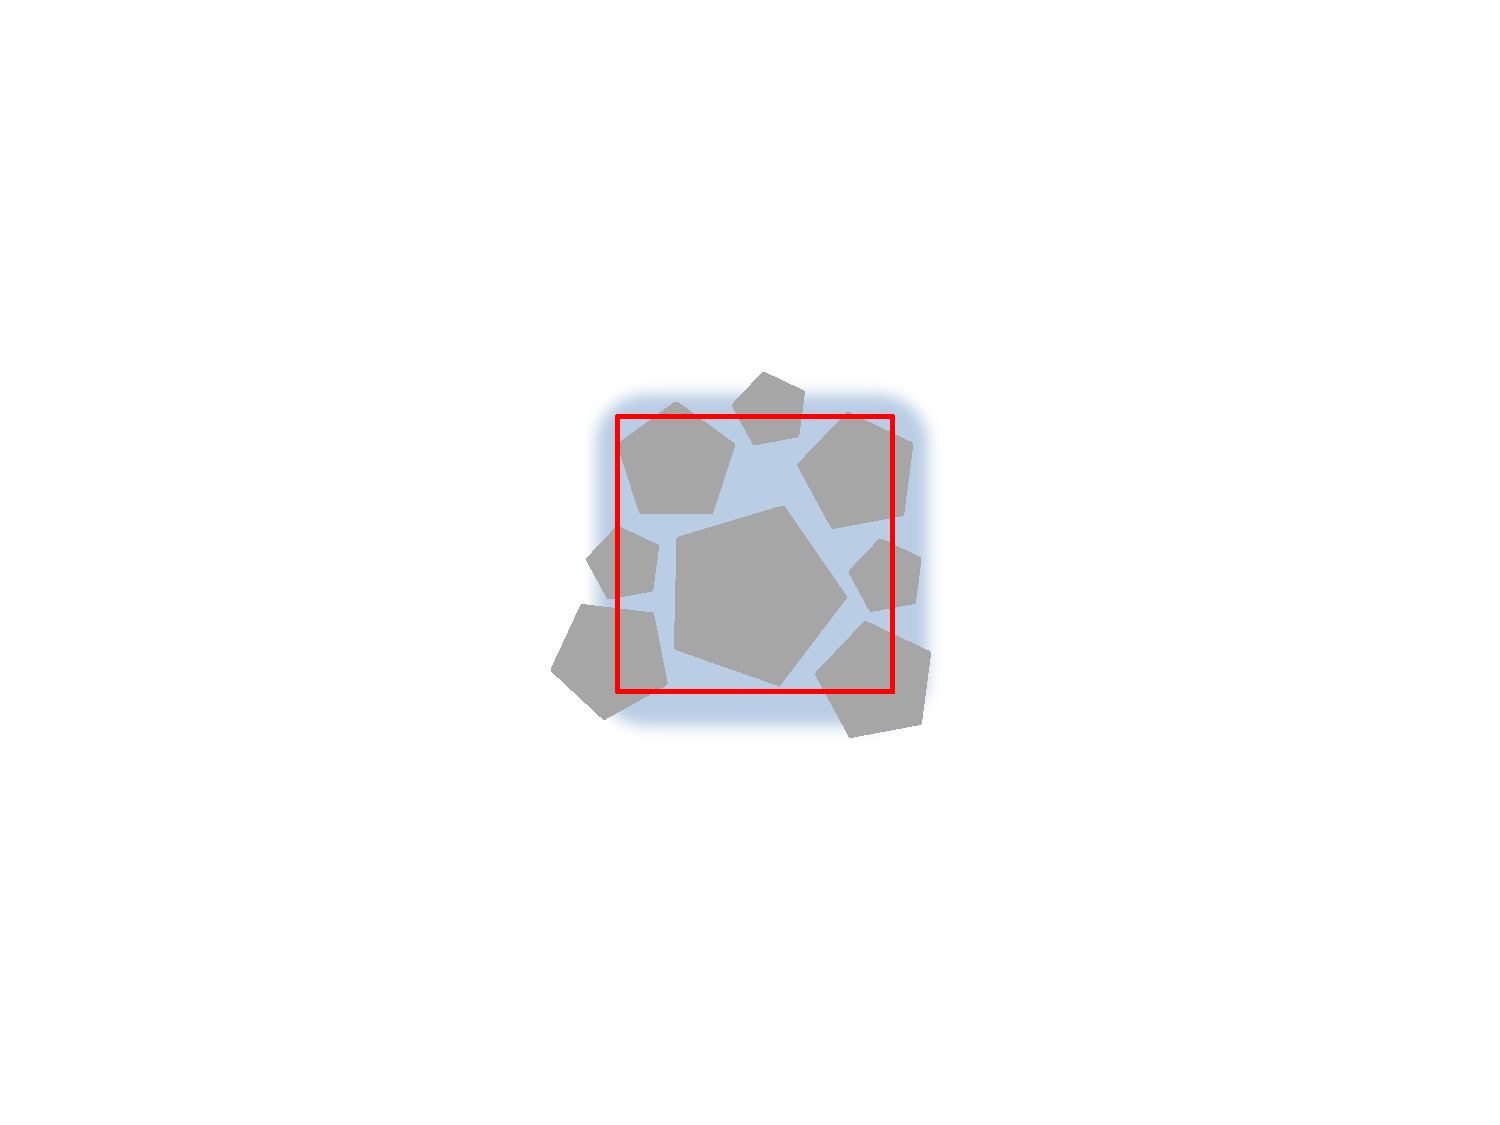
\includegraphics[width = 4.0in,trim=180 180 180 180,clip=true]{RVE_fig.pdf}
	\caption{Representative Volume Element}
	\label{fig:RVE}
\end{figure}

We define the Lagrangian porosity $\phi$ to be the ratio of the total porous (fluid) volume in the current configuration, to the total RVE volume in the reference configuration. This definition is suitable for finite deformation kinematics. While the initial Lagrangian porosity $\phi_0$ (the ratio of reference configuration porous volume to reference configuration total RVE volume) will remain constant for all time, $\phi$ may vary with time. If, however, we make the assumption of small deformations, then we may assert the following simplification: $\phi(t) = \phi_0 \forall t$.

We invoke the notion of a solid `skeleton' being comprised of only the solid phase within the RVE, absent of the saturating fluid. The deformation of the solid `skeleton' will be described by the displacement field $\mathbf{u}(\mathbf{x})$, which will be defined for all spatial coordinates $\mathbf{x}$ contained within the domain of the continuum body $B$ being considered. The fluid phase is assumed to move independently of the solid skeleton, with its motion being governed by the equation of fluid continuity.

For the sake of simplicity, we will assume that the skeleton undergoes only small deformations. Therefore, the linearized strain tensor $\varepsilon_{ij}$ will be defined as the macroscopic strain of the skeleton, such that
\begin{equation}
	\varepsilon_{ij} = \frac{1}{2} (u_{i,j} + u_{j,i})
\end{equation}
If we consider only the solid phase within the RVE, we may propose an `effective' skeleton stress $\sigma'_{ij}$ as
\begin{equation}
	\sigma'_{ij} = C_{ijkl} \varepsilon_{kl}
\end{equation}
where $C_{ijkl}$ is the skeleton stiffness tensor. The effective stress may be thought of as a macroscopic quantity. In general, however, the effective skeleton stress does not fully describe the true (microscopic) stress in the solid constituent, which will depend on the pore structure of the material. In essence, the effective stress may be thought of as a volume averaging over the RVE of the true stress in the solid.

If we now consider only the fluid phase within the RVE, we may state the intrinsic pressure in the fluid as $p(\textbf{x})$ $\forall \textbf{x} \in B$. 

We may consider the total stress in the RVE $\sigma_{ij}$ to be the sum of partial stress contributions from both the solid and fluid phases, such that
\begin{equation}
	\sigma_{ij} = \sigma_{ij}^s + \sigma_{ij}^f
\end{equation}
where $\sigma_{ij}^s$ and $\sigma_{ij}^f$ are the stresses within the solid matrix and the fluid which have been \textit{averaged} over the RVE. The fluid stress tensor takes the form
\begin{equation}
	\sigma_{ij}^f = -b_{ij} p
\end{equation}
where $b_{ij}$ is a symmetric rank 2 tensor (generally referred to as Biot's modulus in the poromechanics literature) whose action is to link increments of intrinsic fluid pressure to the total stress in the RVE. In the special case of an isotropic medium, $b_{ij}$ reduces to a spherical tensor, where $b_{11} = b_{22} = b_{33}$, and $b_{ij} = 0$ for $i \neq j$. If we additionally claim that the partial stress contribution from the solid $\sigma_{ij}^s$ is the effective stress $\sigma'_{ij}$, then the total stress in the RVE may be expressed as
\begin{equation}
	\sigma_{ij} = C_{ijkl} \varepsilon_{kl} - b_{ij} p
\end{equation}

The typical equilibrium equation for the RVE may be written as
\begin{equation}
	\sigma_{ij,j} + \rho g_i = \mathbf{0} \quad \forall \mathbf{x} \in B
\end{equation}
where $g_i$ is the body force acting on the RVE, and $\rho$ is the overall mass density per unit of initial RVE volume, defined as
\begin{equation}
	\rho = (1 - \phi_0) \rho^s_0 + \phi \rho^f
\end{equation}
It should be noted that the contribution to the overall mass density from the solid ($(1 - \phi_0) \rho^s_0$) is constant for all time, where $\rho^s_0$ is the intrinsic mass density of the solid in the reference configuration. However, the contribution from the fluid ($\phi \rho^f$) is allowed to vary in time due to both the change in pore volume $\phi$, and the change in the fluid's intrinsic mass density $\rho^f$. In our treatment of poromechanics, we will consider only quasi-static equilibrium, acting under the assumption that the dynamics of the problems that we seek to model are negligible.

Along a similar train of thought, we assume that the inertia of the fluid will not significantly contribute to the fluid motion, with the flow being predominantly pressure-driven. We will therefore model the \textit{averaged} velocity of the fluid $\mathcal{V}_i$ using Darcy's law
\begin{equation}
	\mathcal{V}_i = - \frac{\kappa_{ij}}{\mu} (p_{,j} - \rho^f g_j )
\end{equation}
where $\mu$ is the fluid viscosity, $\kappa_{ij}$ is the intrinsic permeability of the porous medium, and $\rho^f$ is the fluid density (which may be expressed as a function of $p$.) The hydraulic conductivity of the medium is defined as $k_{ij} = \kappa_{ij}/ \mu$. We notice that the flux rate is governed by a combined fluid potential that accounts for both pressure potential from $\nabla p$, and body force (or gravitational) potential from $\rho^f g_j$. If one were to consider a pressure field set consistent with a hydrostatic pressure field resulting from a constant body force $g_i$, then the resulting combined fluid potential would sum to zero, and thus the flux $\mathcal{V}_i$ would be zero as well (i.e. hydrostatic conditions.) This rationale helps to confirm our intuition of how the fluid should behave in the presence of a body force.

To ensure conservation of fluid mass, we may consider our RVE as a control volume. The fractional volume of fluid contained within this control volume is simply the pore volume $\phi$. Based on the equation of fluid continuity, we may relate the total time rate of change of the fluid volume $\phi$ contained within the RVE to the divergence of the flux rate $\mathcal{V}_i$
\begin{equation}
	\frac{\partial}{\partial t} \phi + \mathcal{V}_{i,i} = 0 \quad \forall \mathbf{x} \in B
\end{equation}
That is to say, the change in fluid volume within the RVE must be balanced by the net volumetric fluid flux into or out of the control volume. However, the above differential equation more strictly enforces this condition to hold point-wise throughout the body, and not just for a specific control volume.

We would like to express the total pore volume $\phi$ in terms of $\mathbf{u}$ and $p$, as these will turn out to be our primary variables. We may use the following relation
\begin{equation}
	\phi = \phi_0 + b_{ij} \varepsilon_{ij} + \frac{p}{M}
\end{equation}
where all variables have been defined previously except for $\frac{1}{M}$, which effectively acts as a fluid capacity parameter. It is analogous to the `volumetric specific storage' in groundwater flow terminology. Intuitively, $\frac{1}{M}$ links increments of fluid pressure to changes in the total pore volume. We also observe that the skeleton dilation influences the pore volume through Biot's modulus.

As stated previously, we will select $\mathbf{u}(\mathbf{x})$ as one of our primary variables. The corresponding boundary and initial conditions on the body $B$ are expressed as follows
\begin{equation}
	u_i = \bar{u}_i \quad on \quad \partial_u B
\end{equation}
\begin{equation}
	\sigma_{ij} n_j = \bar{t}_i \quad on \quad \partial_t B
\end{equation}
\begin{equation}
	u_i (t=0) = u_i^0
\end{equation}
We define $\partial_u B$ and $\partial_t B$ as the parts of the boundary on which prescribed skeleton displacements ($\bar{u}_i$) and prescribed tractions ($\bar{t}_i$) are specified, respectively. $n_j$ is an outward unit surface normal, and $u^0_i$ is the initial skeleton displacement field (at $t=0$.)

We also select $p(\mathbf{x})$ as our other primary variable. The corresponding boundary and initial conditions are
\begin{equation}
	p = \bar{p} \quad on \quad \partial_p B
\end{equation}
\begin{equation}
	\mathcal{V}_i n_i = \bar{\mathcal{V}} \quad on \quad \partial_{\mathcal{V}} B
\end{equation}
\begin{equation}
	p (t=0) = p^0
\end{equation}
We define $\partial_p B$ and $\partial_{\mathcal{V}} B$ as the parts of the boundary on which prescribed fluid pressures ($\bar{p}$) and prescribed normal fluid flux rates ($\bar{\mathcal{V}}$) are specified, respectively. As before, $n_i$ is an outward unit surface normal, and $p^0$ is the initial fluid pressure field (at $t=0$.)

It may be noted that
\begin{equation}
	\partial_u B \cup \partial_{t} B = \partial B \qquad \partial_u B \cap \partial_{t} B = \emptyset
\end{equation}
and
\begin{equation}
	\partial_p B \cup \partial_{\mathcal{V}} B = \partial B \qquad \partial_p B \cap \partial_{\mathcal{V}} B = \emptyset
\end{equation}
where $\partial B$ is the complete boundary of the body $B$. However, it is in general not the case that $\partial_u B = \partial_p B$, nor that $\partial_t B = \partial_{\mathcal{V}} B$. That is to say, the partition of the boundary upon which skeleton displacements and total traction vectors are prescribed is an altogether distinct and separate partition of the boundary from the one upon which fluid pressures and normal fluid fluxes are prescribed. For example, it is entirely possible for $\partial_u B$ to overlap with both $\partial_p B$ and $\partial_{\mathcal{V}} B$.

In practice, the initial conditions would likely be set by selecting a $p^0$ consistent with a hydrostatic pressure distribution, i.e. $p_{,j}^0 = \rho^f g_j$. The resulting $u_i^0$ could then be solved for given this pressure field.

To recapitulate, we now present the equations of poroelasticity in strong form.

\begin{center} \textbf{Governing Equations: Strong Form} \end{center}

Equation of Equilibrium of the Poroelastic Solid:

\begin{equation}
	\sigma_{ij,j} + \rho g_i = 0 \qquad \forall x \in B
\end{equation}

Boundary Conditions for the Poroelastic Solid:

\begin{equation}
	u_i = \bar{u}_i \quad on \quad \partial_u B
\end{equation}
\begin{equation}
	\sigma_{ij} n_j = \bar{t}_i \quad on \quad \partial_t B
\end{equation}

Initial Conditions for the Poroelastic Solid:

\begin{equation}
	u_i (t=0) = u_i^0
\end{equation}

Equation of Compressible Fluid Flow in a Porous Medium:

\begin{equation}
	\frac{\partial}{\partial t} \phi + \mathcal{V}_{i,i} = 0 \qquad \forall x \in B
\end{equation}

Boundary Conditions for the Compressible Fluid:

\begin{equation}
	p = \bar{p} \quad on \quad \partial_p B
\end{equation}
\begin{equation}
	\mathcal{V}_i n_i = \bar{\mathcal{V}} \quad on \quad \partial_{\mathcal{V}} B
\end{equation}

Initial Conditions for the Compressible Fluid:
\begin{equation}
	p (t=0) = p^0
\end{equation}

Constitutive Relations for the Poroelastic Solid:
\begin{equation}
	\sigma_{ij} = C_{ijkl} \varepsilon_{kl} - b_{ij} p
\end{equation}
\begin{equation}
	\varepsilon_{ij} = \frac{1}{2} (u_{i,j}+u_{j,i})
\end{equation}

Constitutive Relations for the Compressible Fluid:
\begin{equation}
	\phi = \phi_0 + b_{ij} \varepsilon_{ij} + \frac{p}{M}
	\label{eq:phi}
\end{equation}
\begin{equation}
	\mathcal{V}_i = -k_{ij} ( p_{,j} - \rho^f g_j )
\end{equation}

In what follows, we will present the statement of the equivalent weak form problem statement, along with a derivation of the discrete-in-time equations of poroelasticity. Finally, we will use a Galerkin approximation of these equations to obtain the complete system of finite element equations, presented in matrix form.

\begin{center} \textbf{Generalized Weak Form Problem Statement} \end{center}
Define:
\begin{equation}
	u_i \in \mathcal{S} = \{ u_i | u_i \in H^1 (B), u_i = \bar{u}_i \quad on \quad \partial_u B \}
\end{equation}
\begin{equation}
	v_i \in V = \{ v_i | v_i \in H^1 (B), v_i = 0 \quad on \quad \partial_u B \}
\end{equation}
and
\begin{equation}
	p_i \in \mathcal{T} = \{ p | p \in H^1 (B), p = \bar{p} \quad on \quad \partial_p B \}
\end{equation}
\begin{equation}
	q_i \in \mathcal{Q} = \{  q | q \in H^1 (B), q = 0 \quad on \quad \partial_p B \}
\end{equation}
Find $u_i \in \mathcal{S}$ and $p \in \mathcal{T}$ such that:
\begin{equation}
	\int_B \sigma_{ij} v_{i,j} dv = \int_{\partial_t B} \bar{t}_i v_i da + \int_B \rho g_i v_i dv \quad \forall v_i \in V
\end{equation}
and
\begin{equation}
	\int_B \mathcal{V}_i q_{,i} dv = \int_{\partial_{\mathcal{V}} B} \bar{\mathcal{V}} q da + \int_B \frac{\partial \phi}{\partial t} q dv \quad \forall q \in \mathcal{Q}
\end{equation}

\begin{center} \textbf{Derivation of the Discrete-in-Time Equations} \end{center}
Substitute the constitutive relations for the fluid and the solid into each integral statement
\begin{equation}
	\int_B \left[ C_{ijkl} \{ \frac{1}{2} (u_{k,l}+u_{l,k}) \} - b_{ij} p \right] v_{i,j} dv = \int_{\partial_t B} \bar{t}_i v_i da + \int_B \rho g_i v_i dv \quad \forall v_i \in V
\end{equation}
\begin{equation}
	\int_B \left[ -k_{ij} ( p_{,j} - \rho^f g_j ) \right] q_{,i} dv = \int_{\partial_{\mathcal{V}} B} \bar{\mathcal{V}} q da + \int_B \frac{\partial}{\partial t} ( \phi_0 + b_{ij} \epsilon_{ij} + \frac{p}{M} ) q dv \quad \forall q \in \mathcal{Q}
\end{equation}
simplifying,
\begin{equation}
	\int_B v_{i,j} C_{ijkl} u_{k,l} dv - \int_B v_{i,j} b_{ij} p dv = \int_{\partial_t B} v_i \bar{t}_i da + \int_B v_i \rho g_i dv \quad \forall v_i \in V
\end{equation}
\begin{equation}
	- \int_B q_{,i} k_{ij} p_{,j} dv - \int_B q \frac{\partial}{\partial t} ( b_{ij} u_{i,j} + \frac{p}{M} ) dv= \int_{\partial_{\mathcal{V}} B} q \bar{\mathcal{V}} da - \int_B q_{,i} k_{ij} \rho^f g_j dv \quad \forall q \in \mathcal{Q}
	\label{eq:weakpressure}
\end{equation}
Integrate each of the above equations with respect to time from $t_m$ to $t_{m+1}$
\begin{eqnarray}
	\int_{t_m}^{t_{m+1}} \left[ \int_B v_{i,j} C_{ijkl} u_{k,l} dv - \int_B v_{i,j} b_{ij} p dv \right] dt ... \nonumber \\
	... = \int_{t_m}^{t_{m+1}} \left[ \int_{\partial_t B} v_i \bar{t}_i da + \int_B v_i \rho g_i dv \right] dt \quad \forall v_i \in V
\end{eqnarray}
\begin{eqnarray}
	\int_{t_m}^{t_{m+1}} \left[ - \int_B q_{,i} k_{ij} p_{,j} dv - \int_B q \frac{\partial}{\partial t} ( b_{ij} u_{i,j} + \frac{p}{M} ) dv \right] dt ... \nonumber \\
	... = \int_{t_m}^{t_{m+1}} \left[ \int_{\partial_{\mathcal{V}} B} q \bar{\mathcal{V}} da - \int_B q_{,i} k_{ij} \rho^f g_j dv \right] dt \quad \forall q \in \mathcal{Q} 
\end{eqnarray}
and define
\begin{equation}
	\Delta t = t_{m+1} - t_m
\end{equation}
We propose an approximate integration scheme (generalized trapezoidal rule) as follows for a general function of time, $f(t)$
\begin{equation}
	\int_{t_m}^{t_{m+1}} f(t) dt \approx \left[ \frac{1}{2} (1 + \theta) f^{(m+1)} + \frac{1}{2} (1 - \theta) f^{(m)} \right] \Delta t = f^{(m,\theta)} \Delta t
\end{equation}
where $\theta = +1$ corresponds to the Backward Euler method, $\theta = -1$ corresponds to the Forward Euler method, and $\theta = 0$ corresponds to the Crank-Nicolson method. Applying this rule to our integral statements from before, we obtain the discrete-in-time weak form equations
\begin{eqnarray}
	\int_B v_{i,j} C_{ijkl}^{(m,\theta)} u_{k,l}^{(m,\theta)} dv - \int_B v_{i,j} b_{ij}^{(m,\theta)} p^{(m,\theta)} dv ... \nonumber \\
	... = \int_{\partial_t B} v_i \bar{t}_i^{(m,\theta)} da + \int_B v_i \rho^{(m,\theta)} g_i dv \quad \forall v_i \in V
\end{eqnarray}
\begin{eqnarray}
	- \Delta t \int_B q_{,i} k_{ij}^{(m,\theta)} p_{,j}^{(m,\theta)} dv - \int_B q b_{ij}^{(m+1)} u_{i,j}^{(m+1)} dv - \int_B q \frac{p^{(m+1)}}{M^{(m+1)}} dv ... \nonumber \\
	... = \Delta t \left[ \int_{\partial_{\mathcal{V}} B} q \bar{\mathcal{V}}^{(m,\theta)} da - \int_B q_{,i} k_{ij}^{(m,\theta)} \rho^{f (m,\theta)} g_j dv \right] ... \nonumber \\
	... - \int_B q b_{ij}^{(m)} u_{i,j}^{(m)} dv - \int_B q \frac{p^{(m)}}{M^{(m)}} dv \quad \forall q \in \mathcal{Q}
\end{eqnarray}

\begin{center} \textbf{Galerkin Approximation} \end{center}
In what follows, we will adopt a similar notational scheme as in reference [5]. We now wish to find an approximate solution, $u^h_i \in \mathcal{S}^h \subset \mathcal{S}$ and $p^h \in \mathcal{T}^h \subset \mathcal{T}$ such that
\begin{equation}
	\mathbf{u}^h = \sum_{a \in \eta_0} \Phi_a \mathbf{u}_a + \sum_{a \in \eta_u} \Phi_a \bar{\mathbf{u}}_a, \qquad p^h = \sum_{a \in \zeta_0} \hat{\Phi}_a p_a + \sum_{a \in \zeta_p} \hat{\Phi}_a \bar{p}_a
\end{equation}
\begin{equation}
	\mathbf{v}^h = \sum_{a \in \eta_0} \Phi_a \mathbf{v}_a, \qquad q^h = \sum_{a \in \zeta_0} \hat{\Phi}_a q_a
\end{equation}
with the following definitions for the sets of nodes, $a$. Note that the sets $\eta_0$ and $\eta_u$ are defined independently from $\zeta_0$ and $\zeta_p$.
\begin{itemize}
	\item[$\eta_0$] The set of nodes without prescribed skeleton displacements
	\item[$\eta_u$] The set of nodes with prescribed skeleton displacements, $\bar{\mathbf{u}}$
	\item[$\zeta_0$] The set of nodes without prescribed fluid pressure
	\item[$\zeta_p$] The set of nodes with prescribed fluid pressure, $\bar{p}$
\end{itemize}
Henceforth, we shall adopt matrix and vector representations for all quantities, with the stress and strain vectors arranged according to Voigt notation. It therefore becomes of interest to investigate the following quantities
\begin{equation}
	\mathbf{\varepsilon} = \sum_{a} \mathbf{B}_a \mathbf{u}_a, \qquad \nabla \cdot p = \sum_{a} \hat{\mathbf{B}}_a p_a
\end{equation}
where we define $\mathbf{B}_a$ and $\hat{\mathbf{B}}_a$ (in three spatial dimensions) as follows
\begin{equation}
	\mathbf{B}_a = \left[
	\begin{array}{ccc}
		\Phi_{a,1} & 0 & 0 \\
		0 & \Phi_{a,2} & 0 \\
		0 & 0 & \Phi_{a,3} \\
		0 & \Phi_{a,3} & \Phi_{a,2} \\
		\Phi_{a,3} & 0 & \Phi_{a,1} \\
		\Phi_{a,2}& \Phi_{a,1} & 0 
	\end{array} \right]
	\qquad
	\hat{\mathbf{B}}_a = \left[
	\begin{array}{c}
		\hat{\Phi}_{a,1} \\
		\hat{\Phi}_{a,2} \\
		\hat{\Phi}_{a,3}
	\end{array} \right]
\end{equation}
We shall also recast the `skeleton' modulus tensor, $C_{ijkl}$, as the canonical modulus matrix, $\mathbf{D}$. Further, we will rearrange the Biot modulus, $b_{ij}$, into the form of a column vector, $\mathbf{b}$, as shown below (in three spatial dimensions)
\begin{equation}
	\mathbf{b} = \left[
	\begin{array}{c}
		b_{11} \\
		b_{22} \\
		b_{33} \\
		b_{23} \\
		b_{13} \\
		b_{12}
	\end{array} \right]
\end{equation}
with these definitions, we may now express the Galerkin approximation to the weak form as follows
\begin{eqnarray}
	 \sum_{b \in \eta_0} \bigg( \int_B \mathbf{B}_a^T \mathbf{D}^{(m,\theta)} \mathbf{B}_b dv \bigg) \mathbf{u}_b^{(m,\theta)} + \sum_{b \in \eta_u} \bigg( \int_B \mathbf{B}_a^T \mathbf{D}^{(m,\theta)} \mathbf{B}_b dv \bigg) \bar{\mathbf{u}}_b^{(m,\theta)} ... \nonumber \\
	... - \sum_{b \in \zeta_0} \bigg( \int_B \mathbf{B}_a^T \mathbf{b}^{(m,\theta)} \hat{\Phi}_b dv \bigg) p_b^{(m,\theta)} - \sum_{b \in \zeta_p} \bigg( \int_B \mathbf{B}_a^T \mathbf{b}^{(m,\theta)} \hat{\Phi}_b dv \bigg) \bar{p}_b^{(m,\theta)} ... \nonumber \\
	... = \int_{\partial_t B} \Phi_a \bar{\mathbf{t}}^{(m,\theta)} da + \int_B \Phi_a \rho^{(m,\theta)} \mathbf{g} dv \quad \forall a \in \eta_0
\end{eqnarray}
\begin{eqnarray}
	\Delta t \left[ - \sum_{b \in \zeta_0} \bigg( \int_B \hat{\mathbf{B}}_a^T \mathbf{k}^{(m,\theta)} \hat{\mathbf{B}}_b dv \bigg) p_b^{(m,\theta)} - \sum_{b \in \zeta_p} \bigg(  \int_B \hat{\mathbf{B}}_a^T \mathbf{k}^{(m,\theta)} \hat{\mathbf{B}}_b dv \bigg) \bar{p}_b^{(m,\theta)} \right] ... \nonumber \\
	... - \sum_{b \in \eta_0} \bigg( \int_B \hat{\Phi}_a \mathbf{b}^{T (m+1)} \mathbf{B}_b dv \bigg) \mathbf{u}_b^{(m+1)} - \sum_{b \in \eta_u} \bigg( \int_B \hat{\Phi}_a \mathbf{b}^{T (m+1)} \mathbf{B}_b dv \bigg) \bar{\mathbf{u}}_b^{(m+1)} ... \nonumber \\
	... - \sum_{b \in \zeta_0} \bigg( \int_B \hat{\Phi}_a M^{-1 (m+1)} \hat{\Phi}_b dv \bigg) p_b^{(m+1)} - \sum_{b \in \zeta_p} \bigg(  \int_B \hat{\Phi}_a M^{-1 (m+1)} \hat{\Phi}_b dv \bigg) \bar{p}_b^{(m+1)} ... \nonumber \\
	... = \Delta t \left[ \int_{\partial_{\mathcal{V}} B} \hat{\Phi}_a \bar{\mathcal{V}}^{(m,\theta)} da - \int_B \hat{\mathbf{B}}_a^T \mathbf{k}^{(m,\theta)} \rho^{f (m,\theta)} \mathbf{g} dv \right] ... \nonumber \\
	... - \sum_{b \in \eta_0} \bigg( \int_B \hat{\Phi}_a \mathbf{b}^{T (m)} \mathbf{B}_b dv \bigg) \mathbf{u}_b^{(m)} - \sum_{b \in \eta_u} \bigg( \int_B \hat{\Phi}_a \mathbf{b}^{T (m)} \mathbf{B}_b dv \bigg) \bar{\mathbf{u}}_b^{(m)} ... \nonumber \\
	... - \sum_{b \in \zeta_0} \bigg( \int_B \hat{\Phi}_a M^{-1 (m)} \hat{\Phi}_b dv \bigg) p_b^{(m)} - \sum_{b \in \zeta_p} \bigg(  \int_B \hat{\Phi}_a M^{-1 (m)} \hat{\Phi}_b dv \bigg) \bar{p}_b^{(m)} \quad \forall a \in \zeta_0
\end{eqnarray}
We can simplify these expressions by introducing the following notation for the integral statements
\begin{equation}
	\mathbf{K_{uu}}_{ab}^{(m)} = \int_B \mathbf{B}_a^T \mathbf{D}^{(m)} \mathbf{B}_b dv \qquad ( 3 \times 3 )
	\label{eq:Kuu}
\end{equation}
\begin{equation}
	\mathbf{K_{up}}_{ab}^{(m)} = \int_B \mathbf{B}_a^T \mathbf{b}^{(m)} \hat{\Phi}_b dv \qquad ( 3 \times 1 )
\end{equation}
\begin{equation}
	\mathbf{K_{pu}}_{ab}^{(m)} = \int_B \hat{\Phi}_a \mathbf{b}^{T (m)} \mathbf{B}_b dv \qquad ( 1 \times 3 )
\end{equation}
\begin{equation}
	{K_{pp}}_{ab}^{(m)} = \int_B \hat{\mathbf{B}}_a^T \mathbf{k}^{(m)} \hat{\mathbf{B}}_b dv \qquad ( 1 \times 1 )
\end{equation}
\begin{equation}
	{M_{pp}}_{ab}^{(m)} = \int_B \hat{\Phi}_a M^{-1 (m)} \hat{\Phi}_b dv \qquad ( 1 \times 1 )
	\label{eq:Mpp}
\end{equation}
this yields
\begin{eqnarray}
	 \sum_{b \in \eta_0} \mathbf{K_{uu}}_{ab}^{(m,\theta)} \mathbf{u}_b^{(m,\theta)} - \sum_{b \in \zeta_0} \mathbf{K_{up}}_{ab}^{(m,\theta)} p_b^{(m,\theta)}  ... \nonumber \\
	... = \int_{\partial_t B} \Phi_a \bar{\mathbf{t}}^{(m,\theta)} da + \int_B \Phi_a \rho^{(m,\theta)} \mathbf{g} dv ... \nonumber \\
	... - \sum_{b \in \eta_u} \mathbf{K_{uu}}_{ab}^{(m,\theta)} \bar{\mathbf{u}}_b^{(m,\theta)} + \sum_{b \in \zeta_p}\mathbf{K_{up}}_{ab}^{(m,\theta)} \bar{p}_b^{(m,\theta)} \quad \forall a \in \eta_0
\end{eqnarray}
\begin{eqnarray}
	 - \sum_{b \in \eta_0} \mathbf{K_{pu}}_{ab}^{(m+1)} \mathbf{u}_b^{(m+1)} - \Delta t \sum_{b \in \zeta_0} {K_{pp}}_{ab}^{(m, \theta)} p_b^{(m,\theta)} - \sum_{b \in \zeta_0} {M_{pp}}_{ab}^{(m+1)} p_b^{(m+1)}  ... \nonumber \\
	... = \Delta t \left[ \int_{\partial_{\mathcal{V}} B} \hat{\Phi}_a \bar{\mathcal{V}}^{(m,\theta)} da - \int_B \hat{\mathbf{B}}_a^T \mathbf{k}^{(m,\theta)} \rho^{f (m,\theta)} \mathbf{g} dv \right] ... \nonumber \\
	... + \sum_{b \in \eta_u} \mathbf{K_{pu}}_{ab}^{(m+1)} \bar{\mathbf{u}}_b^{(m+1)} + \Delta t \sum_{b \in \zeta_p} {K_{pp}}_{ab}^{(m, \theta)} \bar{p}_b^{(m,\theta)} + \sum_{b \in \zeta_p} {M_{pp}}_{ab}^{(m+1)} \bar{p}_b^{(m+1)} ... \nonumber \\
	- \sum_{b \in \eta_0} \mathbf{K_{pu}}_{ab}^{(m)} \mathbf{u}_b^{(m)} - \sum_{b \in \eta_u} \mathbf{K_{pu}}_{ab}^{(m)} \bar{\mathbf{u}}_b^{(m)} - \sum_{b \in \zeta_0} {M_{pp}}_{ab}^{(m)} p_b^{(m)} - \sum_{b \in \zeta_p} {M_{pp}}_{ab}^{(m)} \bar{p}_b^{(m)} \quad \forall a \in \zeta_0
\end{eqnarray}
define contributions to the global forcing/residual vector as
\begin{equation}
	\mathbf{F_{u}}_{a}^{(m)} = \int_{\partial_t B} \Phi_a \bar{\mathbf{t}}^{(m)} da + \int_B \Phi_a \rho^{(m)} \mathbf{g} dv - \sum_{b \in \eta_u} \mathbf{K_{uu}}_{ab}^{(m)} \bar{\mathbf{u}}_b^{(m)} + \sum_{b \in \zeta_p}\mathbf{K_{up}}_{ab}^{(m)} \bar{p}_b^{(m)} \qquad ( 3 \times 1 )
	\label{eq:Fu}
\end{equation}
\begin{equation}
	{F^1_{p}}_{a}^{(m)} = \int_{\partial_{\mathcal{V}} B} \hat{\Phi}_a \bar{\mathcal{V}}^{(m)} da - \int_B \hat{\mathbf{B}}_a^T \mathbf{k}^{(m)} \rho^{f (m)} \mathbf{g} dv + \sum_{b \in \zeta_p} {K_{pp}}_{ab}^{(m)} \bar{p}_b^{(m)} \qquad ( 1 \times 1 )
\end{equation}
\begin{equation}
	{F^2_{p}}_{a}^{(m)} = \sum_{b \in \eta_u} \mathbf{K_{pu}}_{ab}^{(m)} \bar{\mathbf{u}}_b^{(m)} + \sum_{b \in \zeta_p} {M_{pp}}_{ab}^{(m)} \bar{p}_b^{(m)} \qquad ( 1 \times 1 )
	\label{eq:Fp2}
\end{equation}
substituting for the above expressions
\begin{eqnarray}
	 \sum_{b \in \eta_0} \mathbf{K_{uu}}_{ab}^{(m,\theta)} \mathbf{u}_b^{(m,\theta)} - \sum_{b \in \zeta_0} \mathbf{K_{up}}_{ab}^{(m,\theta)} p_b^{(m,\theta)} = \mathbf{F_{u}}_{a}^{(m,\theta)} \quad \forall a \in \eta_0
\end{eqnarray}
\begin{eqnarray}
	 - \sum_{b \in \eta_0} \mathbf{K_{pu}}_{ab}^{(m+1)} \mathbf{u}_b^{(m+1)} - \Delta t \sum_{b \in \zeta_0} {K_{pp}}_{ab}^{(m, \theta)} p_b^{(m,\theta)} - \sum_{b \in \zeta_0} {M_{pp}}_{ab}^{(m+1)} p_b^{(m+1)}  ... \nonumber \\
	... = \Delta t {F^1_{p}}_{a}^{(m,\theta)} + {F^2_{p}}_{a}^{(m+1)} - {F^2_{p}}_{a}^{(m)} - \sum_{b \in \eta_0} \mathbf{K_{pu}}_{ab}^{(m)} \mathbf{u}_b^{(m)} - \sum_{b \in \zeta_0} {M_{pp}}_{ab}^{(m)} p_b^{(m)} \quad \forall a \in \zeta_0
\end{eqnarray}
and expanding the $(m,\theta)$ terms, we obtain
\begin{eqnarray}
	(1+\theta) \left[ \sum_{b \in \eta_0} \mathbf{K_{uu}}_{ab}^{(m+1)} \mathbf{u}_b^{(m+1)} - \sum_{b \in \zeta_0} \mathbf{K_{up}}_{ab}^{(m+1)} p_b^{(m+1)} \right] ... \qquad \qquad \nonumber \\
	... = (1+\theta) \mathbf{F_{u}}_{a}^{(m+1)} + (1-\theta) \left[ \mathbf{F_{u}}_{a}^{(m)} - \sum_{b \in \eta_0} \mathbf{K_{uu}}_{ab}^{(m)} \mathbf{u}_b^{(m)} + \sum_{b \in \zeta_0} \mathbf{K_{up}}_{ab}^{(m)} p_b^{(m)} \right] \quad \forall a \in \eta_0
\end{eqnarray}
\newline
\begin{eqnarray}
	 - \sum_{b \in \eta_0} \mathbf{K_{pu}}_{ab}^{(m+1)} \mathbf{u}_b^{(m+1)} - \sum_{b \in \zeta_0} \bigg( (1+\theta) \frac{\Delta t}{2} {K_{pp}}_{ab}^{(m+1)} + {M_{pp}}_{ab}^{(m+1)} \bigg) p_b^{(m+1)}  ... \nonumber \\
	... = (1+\theta) \frac{\Delta t}{2} {F^1_{p}}_{a}^{(m+1)} + {F^2_{p}}_{a}^{(m+1)} + (1-\theta) \frac{\Delta t}{2} {F^1_{p}}_{a}^{(m)} - {F^2_{p}}_{a}^{(m)} ... \nonumber \\
	... - \sum_{b \in \eta_0} \mathbf{K_{pu}}_{ab}^{(m)} \mathbf{u}_b^{(m)} - \sum_{b \in \zeta_0} \bigg( (\theta-1) \frac{\Delta t}{2} {K_{pp}}_{ab}^{(m)} + {M_{pp}}_{ab}^{(m)} \bigg) p_b^{(m)} \quad \forall a \in \zeta_0
\end{eqnarray}
For $\theta = 0$ (Crank-Nicolson method) we find
\begin{eqnarray}
	\sum_{b \in \eta_0} \mathbf{K_{uu}}_{ab}^{(m+1)} \mathbf{u}_b^{(m+1)} - \sum_{b \in \zeta_0} \mathbf{K_{up}}_{ab}^{(m+1)} p_b^{(m+1)} ... \qquad \qquad \nonumber \\
	... = \mathbf{F_{u}}_{a}^{(m+1)} + \mathbf{F_{u}}_{a}^{(m)} - \sum_{b \in \eta_0} \mathbf{K_{uu}}_{ab}^{(m)} \mathbf{u}_b^{(m)} + \sum_{b \in \zeta_0} \mathbf{K_{up}}_{ab}^{(m)} p_b^{(m)} \quad \forall a \in \eta_0
\end{eqnarray}
\begin{eqnarray}
	 - \sum_{b \in \eta_0} \mathbf{K_{pu}}_{ab}^{(m+1)} \mathbf{u}_b^{(m+1)} - \sum_{b \in \zeta_0} \bigg( \frac{\Delta t}{2} {K_{pp}}_{ab}^{(m+1)} + {M_{pp}}_{ab}^{(m+1)} \bigg) p_b^{(m+1)}  ... \nonumber \\
	... = \frac{\Delta t}{2} {F^1_{p}}_{a}^{(m+1)} + {F^2_{p}}_{a}^{(m+1)} + \frac{\Delta t}{2} {F^1_{p}}_{a}^{(m)} - {F^2_{p}}_{a}^{(m)} ... \nonumber \\
	... - \sum_{b \in \eta_0} \mathbf{K_{pu}}_{ab}^{(m)} \mathbf{u}_b^{(m)} + \sum_{b \in \zeta_0} \bigg( \frac{\Delta t}{2} {K_{pp}}_{ab}^{(m)} - {M_{pp}}_{ab}^{(m)} \bigg) p_b^{(m)} \quad \forall a \in \zeta_0
\end{eqnarray}
The above equations may be cast in matrix form as:
\begin{eqnarray}
	\left[
	\begin{array}{cc}
		\mathbf{K_{uu}} & -\mathbf{K_{up}} \\
		-\mathbf{K_{pu}} & -\bigg( \frac{\Delta t}{2} \mathbf{K_{pp}} + \mathbf{M_{pp}} \bigg)
	\end{array} \right] ^{(m+1)}
	\left[
	\begin{array}{c}
		\mathbf{u} \\
		\mathbf{p}
	\end{array} \right] ^{(m+1)} \ldots \nonumber \\
	\ldots = \left[
	\begin{array}{cc}
		-\mathbf{K_{uu}} & \mathbf{K_{up}} \\
		-\mathbf{K_{pu}} & \bigg( \frac{\Delta t}{2} \mathbf{K_{pp}} - \mathbf{M_{pp}} \bigg)
	\end{array} \right] ^{(m)}
	\left[
	\begin{array}{c}
		\mathbf{u} \\
		\mathbf{p}
	\end{array} \right] ^{(m)} \ldots \nonumber \\
	\ldots + \left[
	\begin{array}{c}
		\mathbf{F_u} \\
		 \bigg( \frac{\Delta t}{2} \mathbf{F^1_{p}} + \mathbf{F^2_{p}} \bigg)
	\end{array} \right] ^{(m+1)} +
	\left[
	\begin{array}{c}
		\mathbf{F_u} \\
		 \bigg( \frac{\Delta t}{2} \mathbf{F^1_{p}} - \mathbf{F^2_{p}} \bigg)
	\end{array} \right] ^{(m)}
	\label{eq:matrixequations1}
\end{eqnarray}
And in terms of the incremental skeleton displacements and fluid pressures, $\hat{\mathbf{u}}$ and $\hat{\mathbf{p}}$
\begin{eqnarray}
	\left[
	\begin{array}{cc}
		\mathbf{K_{uu}} & -\mathbf{K_{up}} \\
		-\mathbf{K_{pu}} & -\bigg( \frac{\Delta t}{2} \mathbf{K_{pp}} + \mathbf{M_{pp}} \bigg)
	\end{array} \right] ^{(m+1)}
	\left[
	\begin{array}{c}
		\hat{\mathbf{u}} \\
		\hat{\mathbf{p}}
	\end{array} \right] ^{(m+1)} \ldots \qquad \qquad \qquad \qquad \qquad \qquad \nonumber \\
	\ldots = \left[
	\begin{array}{cc}
		-\bigg(\mathbf{K_{uu}}^{(m)} + \mathbf{K_{uu}}^{(m+1)} \bigg) & \bigg(\mathbf{K_{up}}^{(m)} + \mathbf{K_{up}}^{(m+1)} \bigg) \\
		-\bigg(\mathbf{K_{pu}}^{(m)} - \mathbf{K_{pu}}^{(m+1)} \bigg) & \bigg( \frac{\Delta t}{2} \mathbf{K_{pp}}^{(m)} - \mathbf{M_{pp}} ^{(m)} + \frac{\Delta t}{2} \mathbf{K_{pp}} ^{(m+1)} + \mathbf{M_{pp}} ^{(m+1)} \bigg)
	\end{array} \right]
	\left[
	\begin{array}{c}
		\mathbf{u} \\
		\mathbf{p}
	\end{array} \right] ^{(m)} \ldots \nonumber \\
	\ldots + \left[
	\begin{array}{c}
		\mathbf{F_u} \\
		 \bigg( \frac{\Delta t}{2} \mathbf{F^1_{p}} + \mathbf{F^2_{p}} \bigg)
	\end{array} \right] ^{(m+1)} +
	\left[
	\begin{array}{c}
		\mathbf{F_u} \\
		 \bigg( \frac{\Delta t}{2} \mathbf{F^1_{p}} - \mathbf{F^2_{p}} \bigg)
	\end{array} \right] ^{(m)} \qquad \qquad \qquad \qquad \qquad \qquad \qquad \nonumber
	\label{eq:matrixequations}
\end{eqnarray}

\section{Development of a Damage Mechanics Model}

The key concept of damage mechanics is to take what one might refer to as a `smeared' representation of the fracture within a given material. Rather than represent discrete cracks within a given medium that has undergone material failure, the effects of cracking within the material are characterized through a homogenized approach, where the extent of material failure is associated with one or more damage parameters. Such parameters may be used to degrade the elastic properties of the material in such as way as to mimic fracture initiation and propagation from a macroscopic viewpoint. The treatment of materials as homogenized continua in damage mechanics is similar in nature to the way that poromechanics describes porous materials at a macroscopic level. As such, the usage of damage mechanics to simulate hydraulic fracture within porous media would seem to be a natural first choice.

However, rather than simply degrading the elastic properties of the porous material, we would also seek to evolve the permeability of the material in an effort to reflect the allowance of fluid to flow through the newly formed cracks in the rock. Heuristically, one might also expect the porosity of the rock to also be affected by the damage incurred within the material. Reference [7] presents a formulation that evolves both the damage and the porosity of the material in a coupled fashion. However, for our applications we will only consider the case of small deformations, such that $\phi \approx \phi_0$.

In what follows, we will pursue the development of an ad hoc damage mechanics scheme involving only a single damage parameter, based in part upon the concept of a corresponding damage law presented in reference [3]. This parameter will be used to evolve the material properties isotropically. More complicated models may consider the incorporation of multiple damage parameters, with a particular interest in degrading the material anisotropically, in an effort to capture the directionality of cracks. This would be a topic for further research.

We propose a damage variable $D$ such that $D \in (0,1]$. For $D = 1$, we may consider the material as being `undamaged.' A $D < 1$ therefore indicates that the material has incurred some amount of damage. We will prohibit $D = 0$ to avoid divide by zero risk, but for the sake of argument, this would correspond to a `fully' damaged material state. As stated previously, we would like the material properties of our poroelastic medium to depend upon the extent of damage in some way. In particular, we will investigate a scheme which allows for the evolution of the elastic properties of the solid skeleton, as well as the intrinsic permeability of the medium. That is to say
\begin{equation}
	\lambda = \lambda (D); \qquad \mu = \mu (D); \qquad \kappa_{ij} = \kappa_{ij} (D)
\end{equation}
For the time being, we will not make a selection as to exact nature of this dependency, which will allow us to develop a sufficiently general single damage variable scheme.

Given the nature of the problem that we would like to model, it is necessary that we select an appropriate failure criterion that is consistent with the behavior of the material. Since the applications that we are interested in are focused around the brittle failure of rock, we pursue a model that satisfies the following goals:
\begin{itemize}
	\item[1] Failure of the material in uniaxial tension should occur at a lower stress than for failure in uniaxial compression.
	\item[2] Failure of the material should be pressure-dependent. That is to say, failure of the material should occur more easily at lower pressures than at higher pressures.
	\item[3] Failure of the material should be controlled predominantly by the deviatoric stress state.
\end{itemize}

Certain key assumptions have been made in enumerating the above goals that deserve clarification. Given that rock is a brittle material, our selection of goal number 1 is unsurprising. However, we suppose that for fractured rock masses at sufficient depths below ground, the overburden of soil will limit the likelihood of the material failing in mode I fracture (see figure \ref{fig:fracturemodes}.) Given the high pressures at the depths being considered for the problems that we would like to model, this is not an unreasonable assumption. Even with the aid of a pressurizing fluid, it has been observed for hydraulic fracturing procedures that the majority of rock failure is attributable to mode II and III fracture. This figures prominently in our assertion of goal number 3. However, we should not diminish the role that the fracturing fluid plays in assisting failure of the material, which is apparent in our statement of goal number 2. It should be the case that the higher fluid pressures will reduce the total rock pressure, allowing for fracture to occur.

\begin{figure} [!ht]
	\centering
	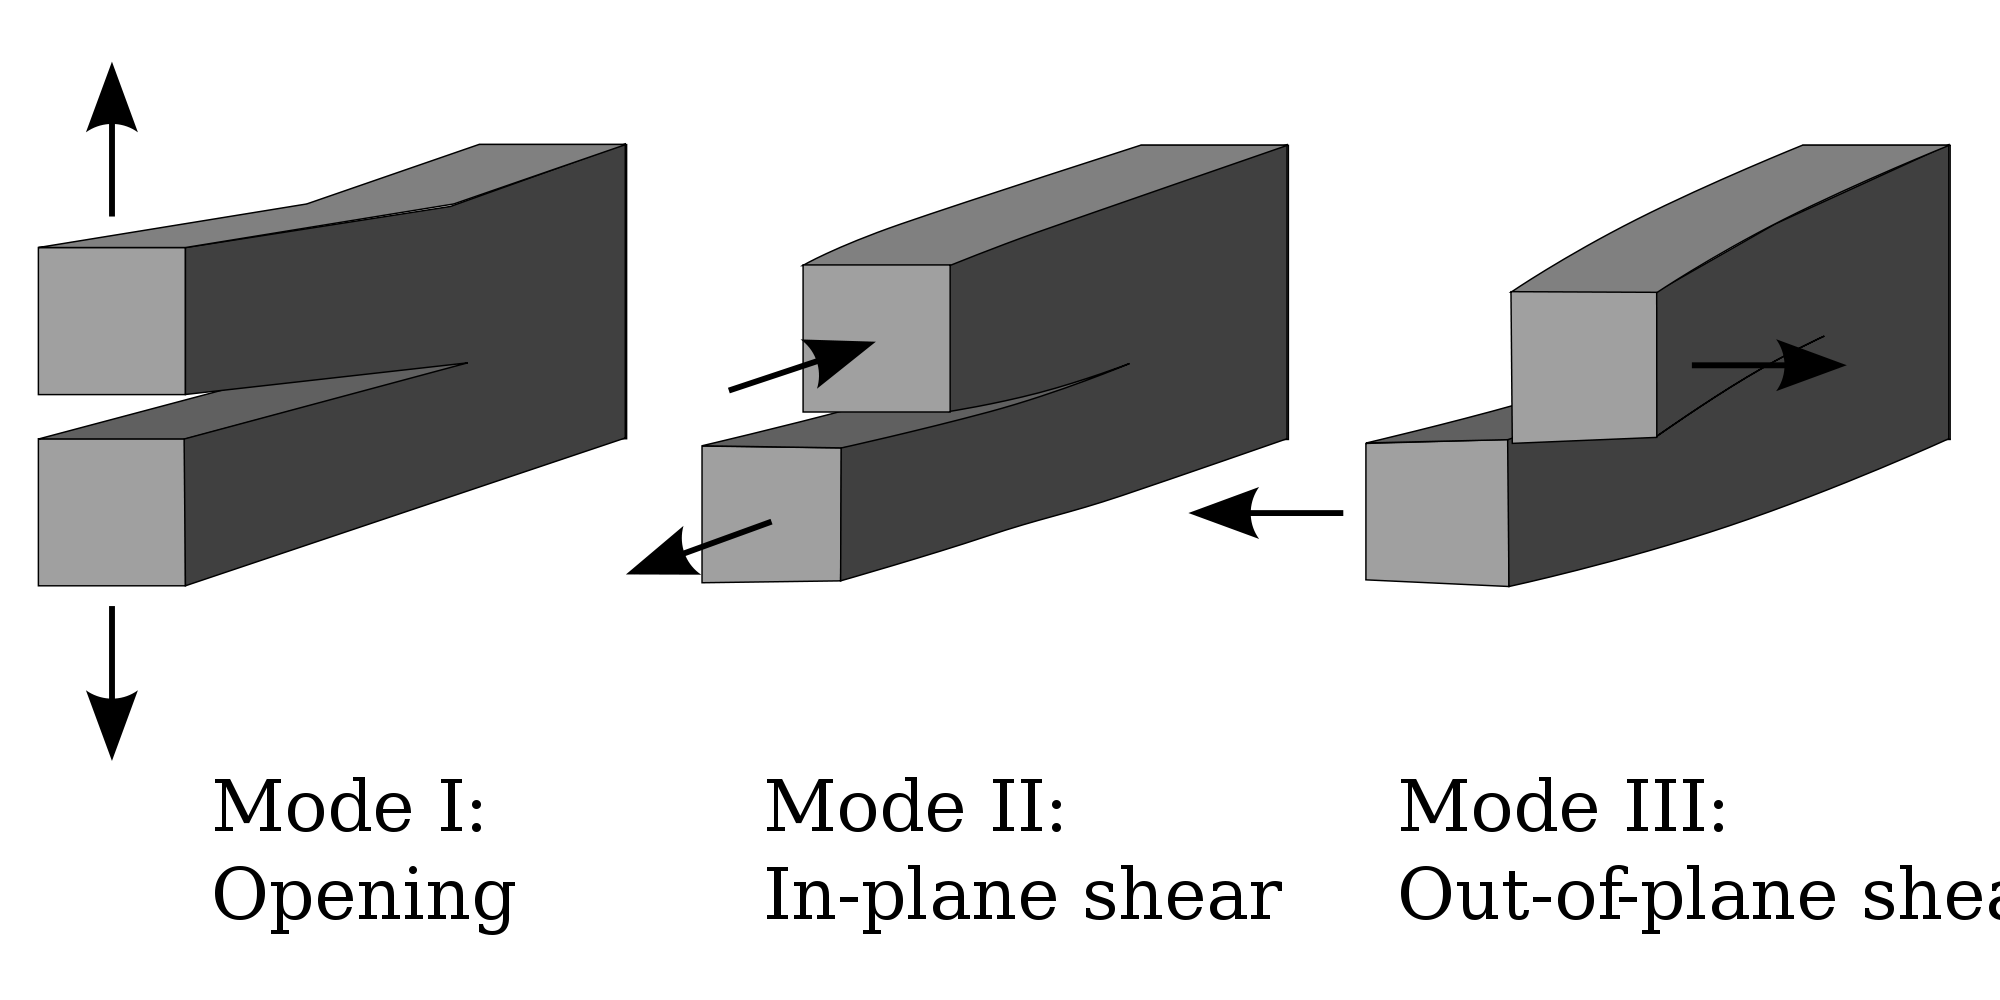
\includegraphics[width = 4.0in,trim=0 150 0 50,clip=true]{fracturemodes.png}
	\caption{Illustration of fracture modes}
	\label{fig:fracturemodes}
\end{figure}

Two possible failure criteria might satisfy the enumerated goals 1 through 3: The Mohr-Coulomb failure criterion, and the Drucker-Prager failure criterion. A detailed description of these criteria may be found in reference [1].  For our purposes, we will select the Drucker-Prager criterion, if for no other reason than its ability to be succinctly expressed as
\begin{equation}
	\sqrt{J_2} = A + B I_1
\end{equation}
where $J_2 = \frac{1}{2} s_{ij} s_{ji}$ is the second invariant of the deviatoric part of the stress ($s_{ij} = \sigma_{ij} - \frac{1}{3} \sigma_{kk} \delta_{ij}$,) $I_1 = \sigma_{kk}$ is the first invariant of the stress $\sigma_{ij}$, and $A$ and $B$ may be written as follows:
\begin{equation}
	A = \frac{2}{\sqrt{3}} \bigg( \frac{\sigma_c \sigma_t}{\sigma_c + \sigma_t} \bigg); \qquad B = \frac{1}{\sqrt{3}} \bigg( \frac{\sigma_t - \sigma_c}{\sigma_c + \sigma_t} \bigg)
\end{equation}
$\sigma_c$ and $\sigma_t$ are defined as the uniaxial failure stresses in compression and tension, respectively. In general, $\sigma_c$ and $\sigma_t$ may differ. In principal stress space, the Drucker-Prager criterion describes a conical surface. Stress states contained within this cone are presumed to be within the elastic range of the material. In our damage model, we will choose to strictly enforce the consistency condition during failure through an appropriate degradation of the material properties.

The distinction should be made at this point that while we are choosing to make use of a failure surface (as is done in the case of plasticity), our approach is more simplistic, in that we are choosing not to decompose the strain into elastic and plastic parts, but rather, we consider the material to remain fully elastic. The basic approach is in many ways similar to the damage model proposed in reference [3]. To enforce the consistency condition, we must permanently degrade the elastic properties of the material. The resulting damaged moduli ($E_D$) will in general be less than the original elastic moduli ($E_0$.) An example of this sort of material behavior for uniaxial monotonic loading and unloading is depicted in figure \ref{fig:uniaxialdamage}.
\begin{figure} [!ht]
	\centering
	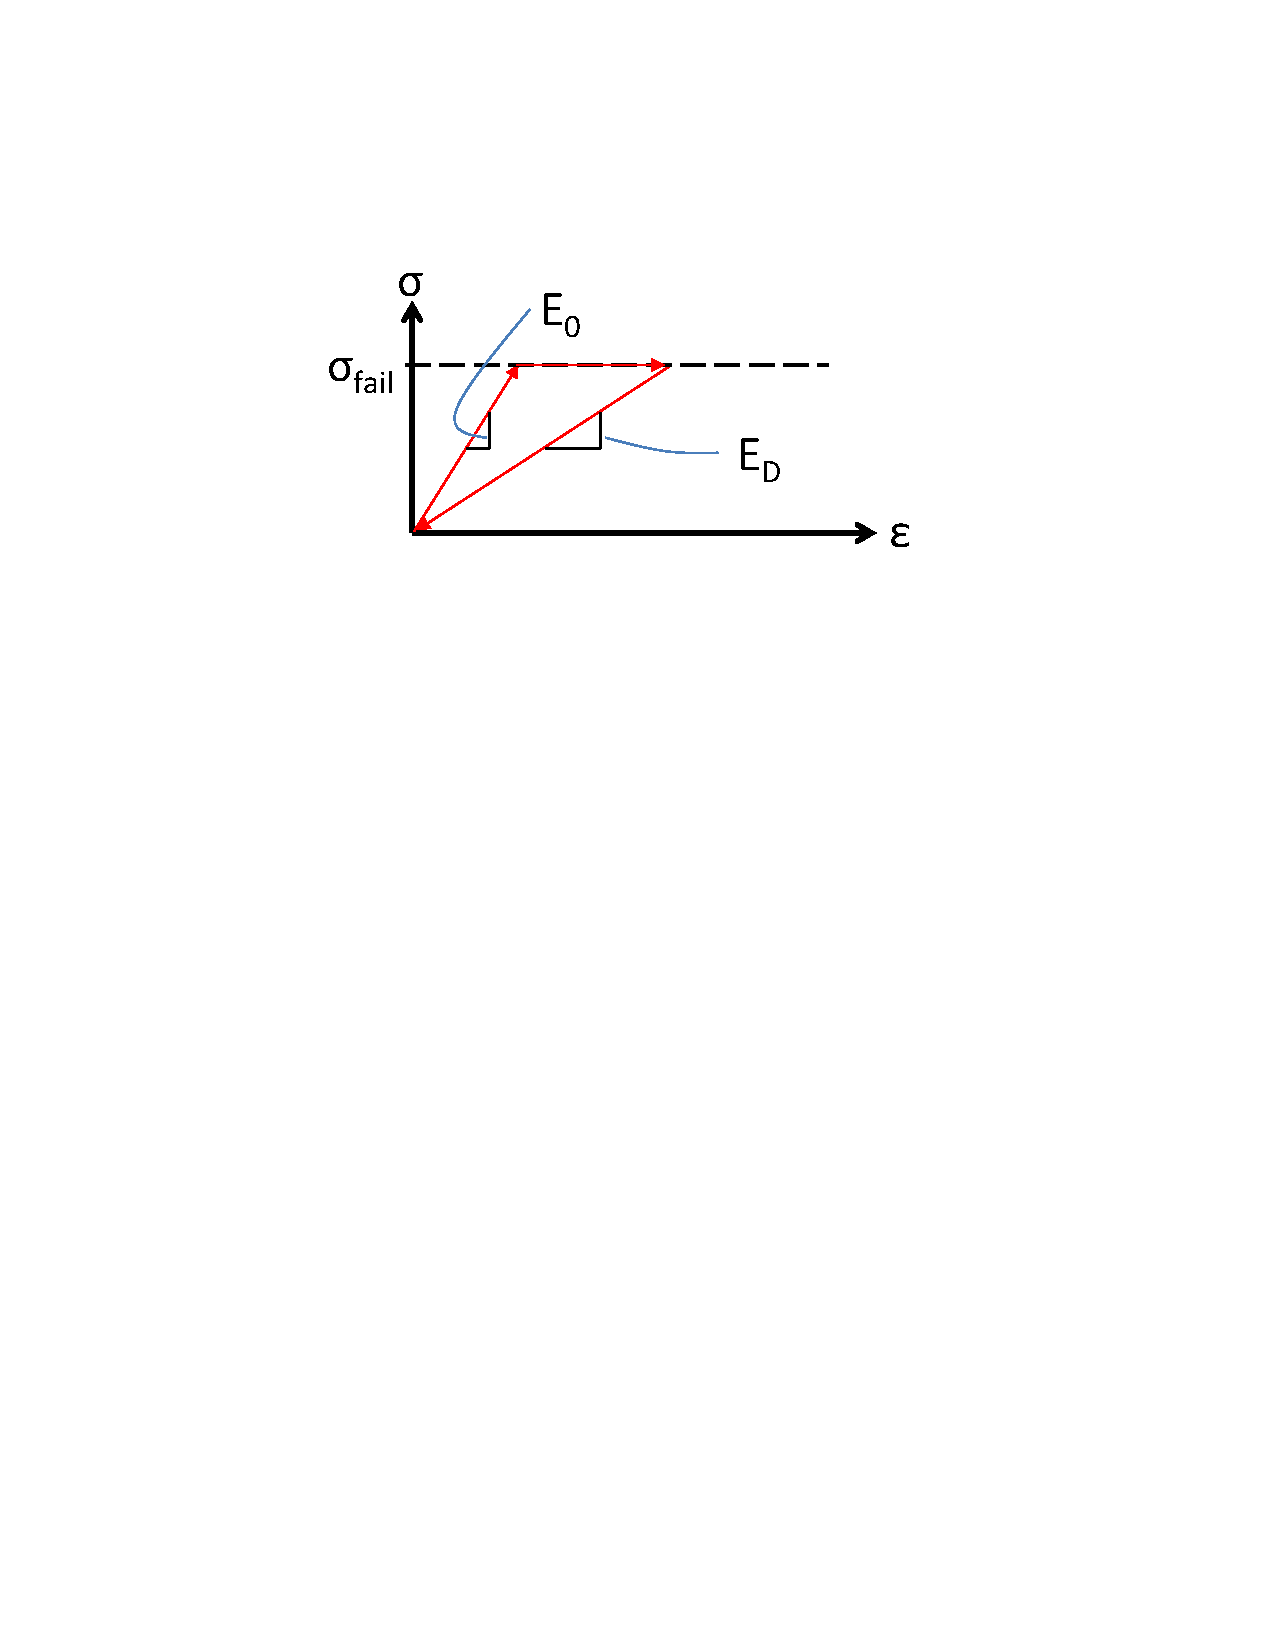
\includegraphics[width = 4.0in,trim=150 530 170 130,clip=true]{uniaxialdamage.pdf}
	\caption{Uniaxial damage model}
	\label{fig:uniaxialdamage}
\end{figure}

For monotonic loading, the model would therefore mimic an elastic-perfectly plastic material. The difference lies in the behavior of the material during unloading. While it is unlikely that the material will behave in exactly this fashion, it is nonetheless a reasonably simple place to start.

We will begin by considering only the porous skeleton of our poroelasticity formulation, in the absence of a saturating fluid. The `effective' stress in the skeleton $\sigma'_{ij} = C_{ijlk} \varepsilon_{kl}$ will be taken as the stress quantity that we will utilize in assessing the consistency condition. The `dry' skeleton will have associated failure stresses in both tension and compression ($\sigma'_c$ and $\sigma'_t$) such that $A$ and $B$ are defined for a given material. We can express the fracture surface as
\begin{equation}
	f(\sigma'_{ij}) = J_2 - (A + B I_1)^2 = 0
\end{equation}
For a given increment of strain, we would like to enforce $f(\sigma'_{ij}) \leq 0$ at the end of a given time step. In a somewhat rudimentary way, we can consider the effective stress $\sigma'_{ij}$ as being dependent upon the elastic properties of the material $\lambda$ and $\mu$, and each of these in turn being dependent upon the amount of damage $D$ incurred by the material. We would therefore like to develop an appropriate evolution law for $D$ that will satisfy the consistency condition ($df = 0$ during failure.)

One method to enforce $f(\sigma_{ij}) = 0$ at the end of a time step would be to adopt the following numerical scheme, equivalent to Newton-Raphson iteration:
\begin{equation}
	D_{i+1} = D_{i} - \frac{f_{i}}{\partial f/ \partial D |_{i}}
	\label{eq:newtonraphson}
\end{equation}
where subscript $i$ denotes an iteration index. It should be emphasized, however, that the end-step value of $D^{(m+1)}$ should be enforced to be less than or equal to the beginning step value of $D^{(m)}$. This requirement comes from the assertion that the extent of damage cannot be reversed. Otherwise, the stress-strain response would be consistent with a non-linear elastic material, which is not what we desire.

Clearly, the adoption of a Newton-Raphson iteration scheme requires that we develop an estimate of the derivative of $f$ with respect to the damage variable $D$. The derivation of this quantity is as follows:

We desire an expression of $J_2$ in terms of the effective stress. We write
\begin{equation}
	J_2 = \frac{1}{2} s_{ij} s_{ji} = \frac{1}{2} \bigg( \sigma'_{ij} - \frac{1}{3} \sigma'_{kk} \delta_{ij} \bigg) \bigg( \sigma'_{ji} - \frac{1}{3} \sigma'_{kk} \delta_{ji} \bigg) = \frac{1}{2} \bigg( \sigma'_{ij} \sigma'_{ji} - \frac{1}{3} (\sigma'_{kk})^2 \bigg)
\end{equation}
We may therefore express $f$ explicitly in terms of the effective stress
\begin{equation}
	f(\sigma'_{ij}) = \frac{1}{2} \sigma'_{ij} \sigma'_{ji} - \bigg( B^2 + \frac{1}{6} \bigg)  (\sigma'_{kk})^2 - 2AB\sigma'_{kk} - A^2 = 0
\end{equation}
If we assume for the sake of simplicity that the material under consideration is both linearly elastic and isotropic, then we may express the effective stress in terms of the total elastic skeleton strain and the Lam\'{e} parameters
\begin{equation}
	\sigma'_{ij} = 2 \mu \varepsilon_{ij} + \lambda \delta_{ij} \varepsilon_{kk}
\end{equation}
so that $f$ may now be expressed in terms of the elastic properties, as well as the increment of skeleton strain
\begin{eqnarray}
	f(\mu,\lambda,\varepsilon_{ij}) = \frac{1}{2} \bigg( 4 \mu^2 \varepsilon_{ij} \varepsilon_{ji} + (4 \mu \lambda + 3 \lambda^2) \varepsilon^2_{kk} \bigg) \\ \nonumber
           - \bigg( B^2 + \frac{1}{6} \bigg) (4 \mu^2 + 12 \mu \lambda + 9 \lambda^2) \varepsilon^2_{kk} - 2AB(2 \mu + 3 \lambda) \varepsilon_{kk} - A^2
\end{eqnarray}
Taking the derivative of $f$ with respect to both $\mu$ and $\lambda$, we obtain
\begin{equation}
	\frac{\partial f}{\partial \mu} = 4 \mu \varepsilon_{ij} \varepsilon_{ji} + 2 \lambda \varepsilon^2_{kk} - \bigg( B^2 + \frac{1}{6} \bigg) (8 \mu + 12 \lambda) \varepsilon^2_{kk} - 4AB \varepsilon_{kk}
\end{equation}
\begin{equation}
	\frac{\partial f}{\partial \lambda} = (2 \mu + 3 \lambda) \varepsilon^2_{kk} - \bigg( B^2 + \frac{1}{6} \bigg) (12 \mu + 18 \lambda) \varepsilon^2_{kk} - 6AB \varepsilon_{kk}
\end{equation}
Using the chain rule of differentiation, we may write
\begin{equation}
	\frac{\partial f}{\partial D} = \frac{\partial f}{\partial \mu} \frac{\partial \mu}{\partial D} + \frac{\partial f}{\partial \lambda} \frac{\partial \lambda}{\partial D}
\end{equation}
All that remains to be done is to fine explicit derivatives of the Lam\'{e} parameters with respect to the damage variable. To do this, however, we must decide how we would like the material parameters to vary with $D$.

We propose the following material degradation scheme:
\begin{equation}
	\mu (D) = \mu_0 D
\end{equation}
\begin{equation}
	\lambda (D) = \lambda_0 + \frac{2}{3} \mu_0 (1 - D)
\end{equation}
which has the property that the bulk modulus $K$ of the solid skeleton is invariant with respect to the damage variable, i.e.
\begin{equation}
	K(D) = \lambda (D) + \frac{2}{3} \mu (D) = \lambda_0 + \frac{2}{3} \mu_0 = K_0 \quad \forall D
\end{equation}
This is desirable because we do not want to degrade the compressibility of the solid constituent. If we assume that the fractured rock mass will experience only positive pressures (given a sufficient depth below ground,) we make the assertion that the fractured rock should still maintain relatively the same compressibility. That is to say, a `crushing' type of failure involving the collapse of pore spaces interior to the rock is not the sort of behavior that we would expect to see in these sorts of problems. This would not, however, be the case if we were to account for dilation of the fractured rock in the event of negative pressures. Otherwise, we should anticipate the shear stiffness of the rock to be linked directly to the extent of damage in the rock (to emulate the behavior of mode II and III fracture.)

Finally, we may express the derivatives of the Lam\'{e} parameters with respect to the damage variable as
\begin{equation}
	\frac{\partial \mu}{\partial D} = \mu_0; \qquad \frac{\partial \lambda}{\partial D} = -\frac{2}{3} \mu_0
\end{equation}
which results in
\begin{equation}
	\frac{\partial f}{\partial D} = \bigg( \frac{\partial f}{\partial \mu} - \frac{2}{3} \frac{\partial f}{\partial \lambda} \bigg) \mu_0
\end{equation}

Up to this point, we have only considered material degradation of the solid matrix. However, we would also like to account for changes in the permeability of the material. We would anticipate it to be the case that the more damaged the material has become, the higher the intrinsic permeability will be. In a very simplistic way, we suggest the following relation
\begin{equation}
	\kappa_{ij} (D) = \frac{\kappa}{D} \delta_{ij}
\end{equation}
where we will now only consider isotropic material behavior, resulting in a scalar valued permeability parameter $\kappa$.

While the total stress $\sigma_{ij}$ in the composite poroelastic material depends upon contributions from both the effective stress in the skeleton as well as the fluid pressure, we remark that failure of the solid material should still only depend upon the effective stress state within the skeleton $\sigma'_{ij}$, and not upon the total stress. This implies that we may directly make use of the previously derived evolution law for $D$. It should be observed, however, that the effective stress state will still depend indirectly upon the fluid pressure. We write the effective stress as follows:
\begin{equation}
	\sigma'_{ij} = \sigma_{ij} + b \delta_{ij} p
\end{equation}
where again, we assume that Biot's modulus is now isotropic, resulting in $b_{ij} = b \delta_{ij}$. For an assumed total stress state of the material that is invariant with respect to time, and for $b > 0$, it is clear that an increase in the fluid pressure $p$ will result in a corresponding increase in the $I1$ effective stress invariant $\sigma'_{kk}$, with the $J_2$ invariant remaining constant. For $B < 0$, which occurs for $\sigma_t < \sigma_c$, it can be seen that this will result in increase in the value of $f$, meaning that failure of the material may be induced through an increase in the hydraulic pressure, which is precisely what we desire.

For a given time step, the numerical scheme that we will choose to adopt will be to first make a prediction of the end-step damage state: $D^{(m+1)} = D^{(m)}$. We can then perform the finite element computations to solve the poroelastic problem for the current time step, given by equation \ref{eq:matrixequations1}. This will provide us with skeleton displacements at the end of the current time step $\textbf{u}^{(m+1)}$, which can be used to compute the end-step skeleton strains $\varepsilon^{(m+1)}_{ij}$. We may then compute
\begin{equation}
	f(D^{(m+1)},\varepsilon^{(m+1)}_{ij}) \qquad and \qquad \frac{\partial f}{\partial D} (D^{(m+1)},\varepsilon^{(m+1)}_{ij})
\end{equation}
which we may use to compute corrected values of the damage variable $D^{(m+1)}_{i+1}$ through equation \ref{eq:newtonraphson}. The corrections could then be modified to satisfy
\begin{equation}
	D^{(m+1)}_{i+1} \in (0,D^{(m)} ]
\end{equation}
such that we prohibit damage reversal from occurring. We may continue to iterate the solution in this manner until we have achieved sufficient convergence in the solution, i.e.
\begin{equation}
	|| D_{i+1} - D_{i} || < tol
	\label{eq:oldnorm}
\end{equation}
or until we have surpassed some maximum number of iterations for the current time step.

\section{MATLAB Implementation}

In an effort to validate our development of the equations of poroelasticity, it became of interest to pursue a two-dimensional, finite element implementation of linear poroelasticity within a simple MATLAB routine. With this in hand, we could explore some simple test problems, and verify if the behavior of the solutions agreed with our intuition.

The simplest implementation that one might conceive of would be to study only isotropic and time invariant material behavior. For the case of an isotropic material, the relations between the poroelastic constants (based on the derivations presented in reference [4]) are as follows:

For Biot's modulus, as we have alluded to in the previous section, we may write
\begin{equation}
	b_{ij} = b \delta_{ij}; \qquad b = 1 - \frac{K}{K_s}
\end{equation}
where $K$ is of course the bulk modulus of the solid skeleton which we are already acquainted with, and $K_s$ is the intrinsic bulk modulus of the solid constituent. It may be noted that for the incorporation of damage evolution into our model, $b(D) = b_0 \forall D$, given that we have imposed the requirement in our damage model that $K(D) = K_0 \forall D$, and because $K_s$ is likewise invariant with respect to $D$.

For the fluid capacity term, we may write
\begin{equation}
	\frac{1}{M} = \frac{1}{N} + \frac{\phi}{K_f}; \qquad \frac{1}{N} = \frac{b - \phi_0}{K_s}
\end{equation}
where $K_f$ is the intrinsic bulk modulus of the fluid. Under the assumption of small deformations, $\phi \approx \phi_0$, and we see that $\frac{1}{M}$ will likewise be invariant with respect to $D$.

As stated previously, the intrinsic permeability, for the case of an isotropic porous medium, may be expressed as
\begin{equation}
	\kappa_{ij} = \kappa \delta_{ij}; \qquad \kappa(D) = \frac{\kappa_0}{D}
\end{equation}
but within the context of our MATLAB implementation, we will impose $D(t) = 1.0 \forall t$, in correspondence with our statement of time invariant material behavior.

For a linearly elastic and isotropic skeleton, the relation between effective stress and skeleton strain (as described in the previous section) is simply
\begin{equation}
	\sigma'_{ij} = 2 \mu \varepsilon_{ij} + \lambda \delta_{ij} \varepsilon_{kk}
\end{equation}
For two-dimensional poroelasticity, we consider only the case of plane strain.

For the finite element formulation, we will consider only the fully-integrated, isoparametric, four-node bilinear quadrilateral element. With each node of the element, we will choose to associate two skeleton displacement degrees of freedom (in the two coordinate directions of the two-dimensional problem,) and a single fluid pressure degree of freedom. In this way, we may utilize the same shape functions and their derivatives to interpolate the values of these quantities on the interior of the element, and to perform the appropriate integrations within the element. We will use Gaussian quadrature to carry out the integrals described in equations \ref{eq:Kuu} through \ref{eq:Mpp} and equations \ref{eq:Fu} through \ref{eq:Fp2}. The linear system described by equation \ref{eq:matrixequations1} can be expressed symbolically as
\begin{equation}
	\mathbf{B} \mathbf{y}^{(m+1)} = \mathbf{A} \mathbf{y}^{(m)} + \mathbf{F}
\end{equation}
The matrices $\mathbf{A}$ and $\mathbf{B}$, as well as the forcing vector $\mathbf{F}$, may be assembled in typical finite element fashion. Once done, we effectively have in hand an implicit update equation for the global vector of unknowns $\mathbf{y}$. For the sake of avoiding the difficulties that can be inherent in iterative solution methods, we will choose to employ a direct linear solution method as a means of obtaining the updated skeleton displacements and pressures at the next time step.

For simplicity, our MATLAB implementation admits only homogeneous essential boundary conditions (i.e. only zero pressures or displacements on $\partial_p B$ and $\partial_u B$, respectively.) Only zero flux boundary conditions were implemented for the natural B.C.s on $\partial_{\mathcal{V}} B$. And, we will restrict the prescribed traction vectors on $\partial_t B$ to be strictly normal to the surface of the body, and constant in magnitude (a pressure-type traction.) Body force has also been neglected, in the interest of observing fluid flow due only to pressure potential.

The visualization capabilities of MATLAB were utilized to the extent that fluid pressure values could be plotted in a colormap on the deformed body. And the displacements and pressures at each time step could then be plotted sequentially to form an animated representation of the time-dependent solution.

We now demonstrate some of the visual results obtained from the MATLAB implementation for a simple test problem: a block of poroelastic material subjected to a sudden increase in confining pressure, with zero displacement and pressure initial conditions. The boundary conditions for this problem are illustrated in figure \ref{fig:exampleproblembcs}.

\begin{figure} [!ht]
	\centering
	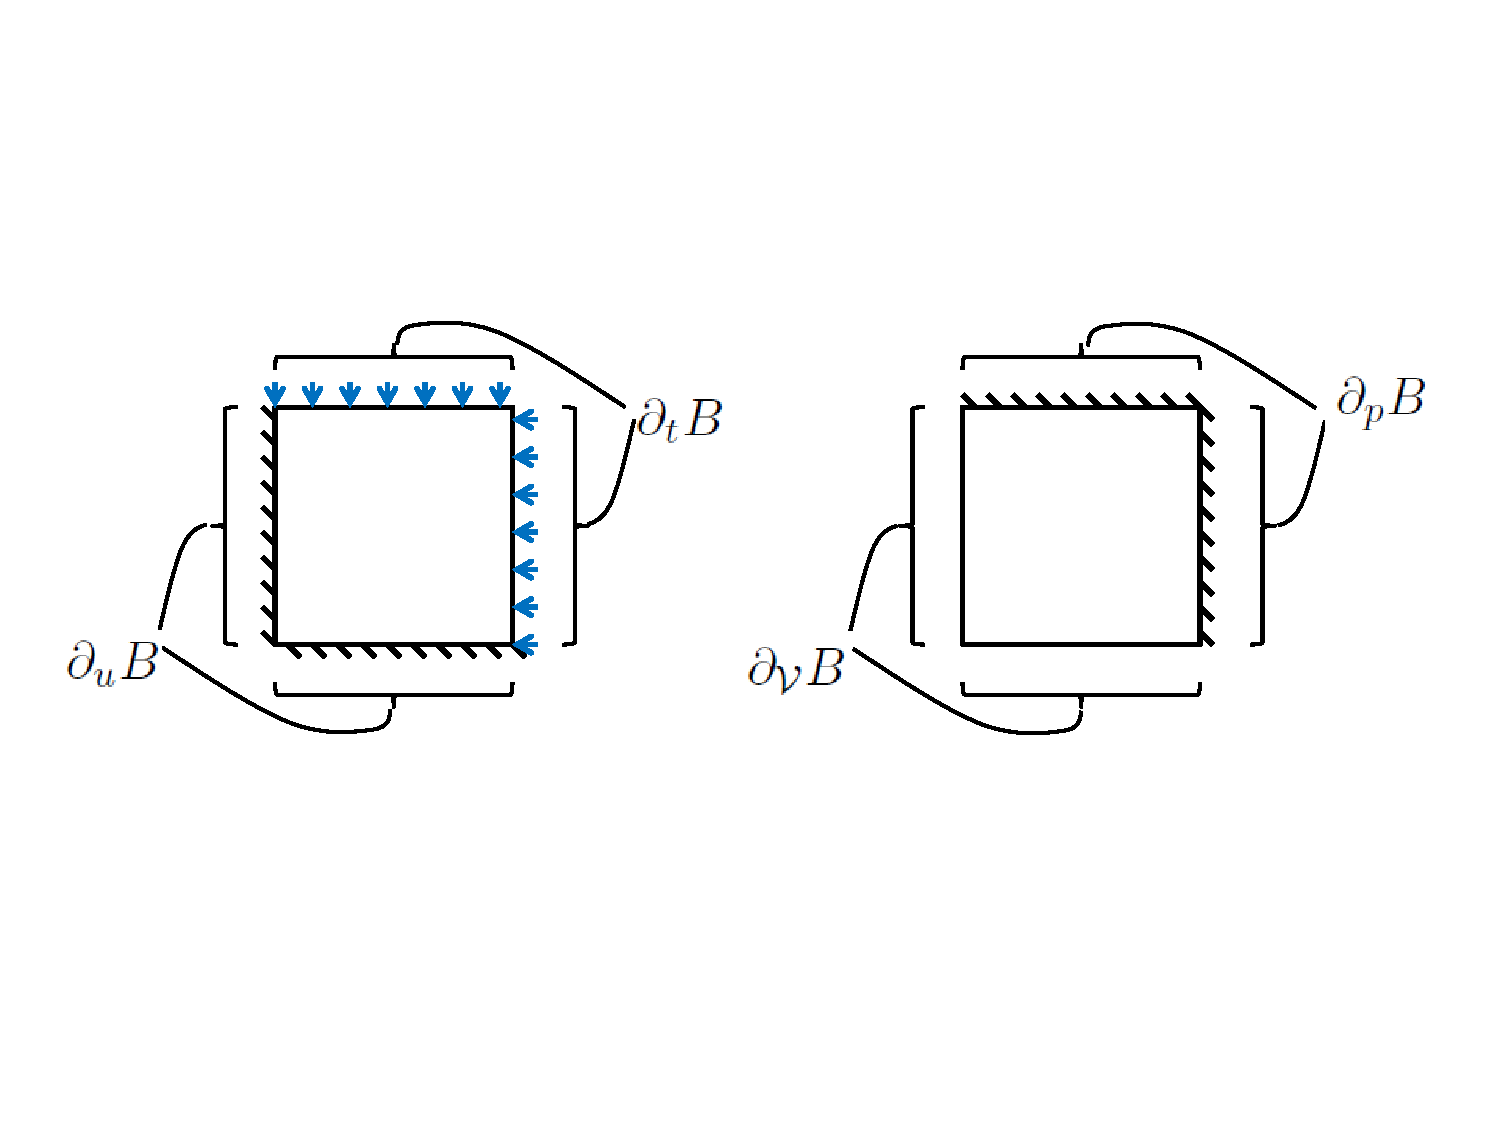
\includegraphics[width = 4.0in,trim=30 180 20 150,clip=true]{exampleproblembcs.pdf}
	\caption{Boundary conditions for MATLAB test problem}
	\label{fig:exampleproblembcs}
\end{figure}

As stated previously, we will only admit homogeneous essential boundary conditions for this problem. In particular, the displacement components normal to the surfaces on $\partial_u B$ are set equal to zero, and the fluid pressure on $\partial_p B$ is set equal to zero as well. Normal fluid fluxes on $\partial_{\mathcal{V}} B$ are likewise equal to zero. The normal (pressure-type) traction boundary condition on $\partial_t B$ will be made a time-varying quantity. Specifically, $t_i = - P(t) n_i$, where $P(t)$ may be thought of as the magnitude of the confining pressure. This test problem makes use of quarter symmetry, in that we are effectively only modeling the top-right corner of a cube of poroelastic material that has been suspended in a zero-pressure fluid, and which is subjected to an increase in the total surrounding pressure on the composite.

The first case that we investigate will have $P(t)$ defined as follows
\begin{equation}
	P(t) =
	\left\{
	\begin{array}{ll}
		P t / t_p & 0 \le t \le t_p \\
		P & t_p < t
	\end{array}
	\right.
	\label{eq:rampload}
\end{equation}
In essence, the confining pressure will ramp up to some constant value of $P$ at time $t_p$. The plotted results are shown in figure \ref{fig:ramptest} for selected values of $t$.
\begin{figure} [!ht]
	\centering
	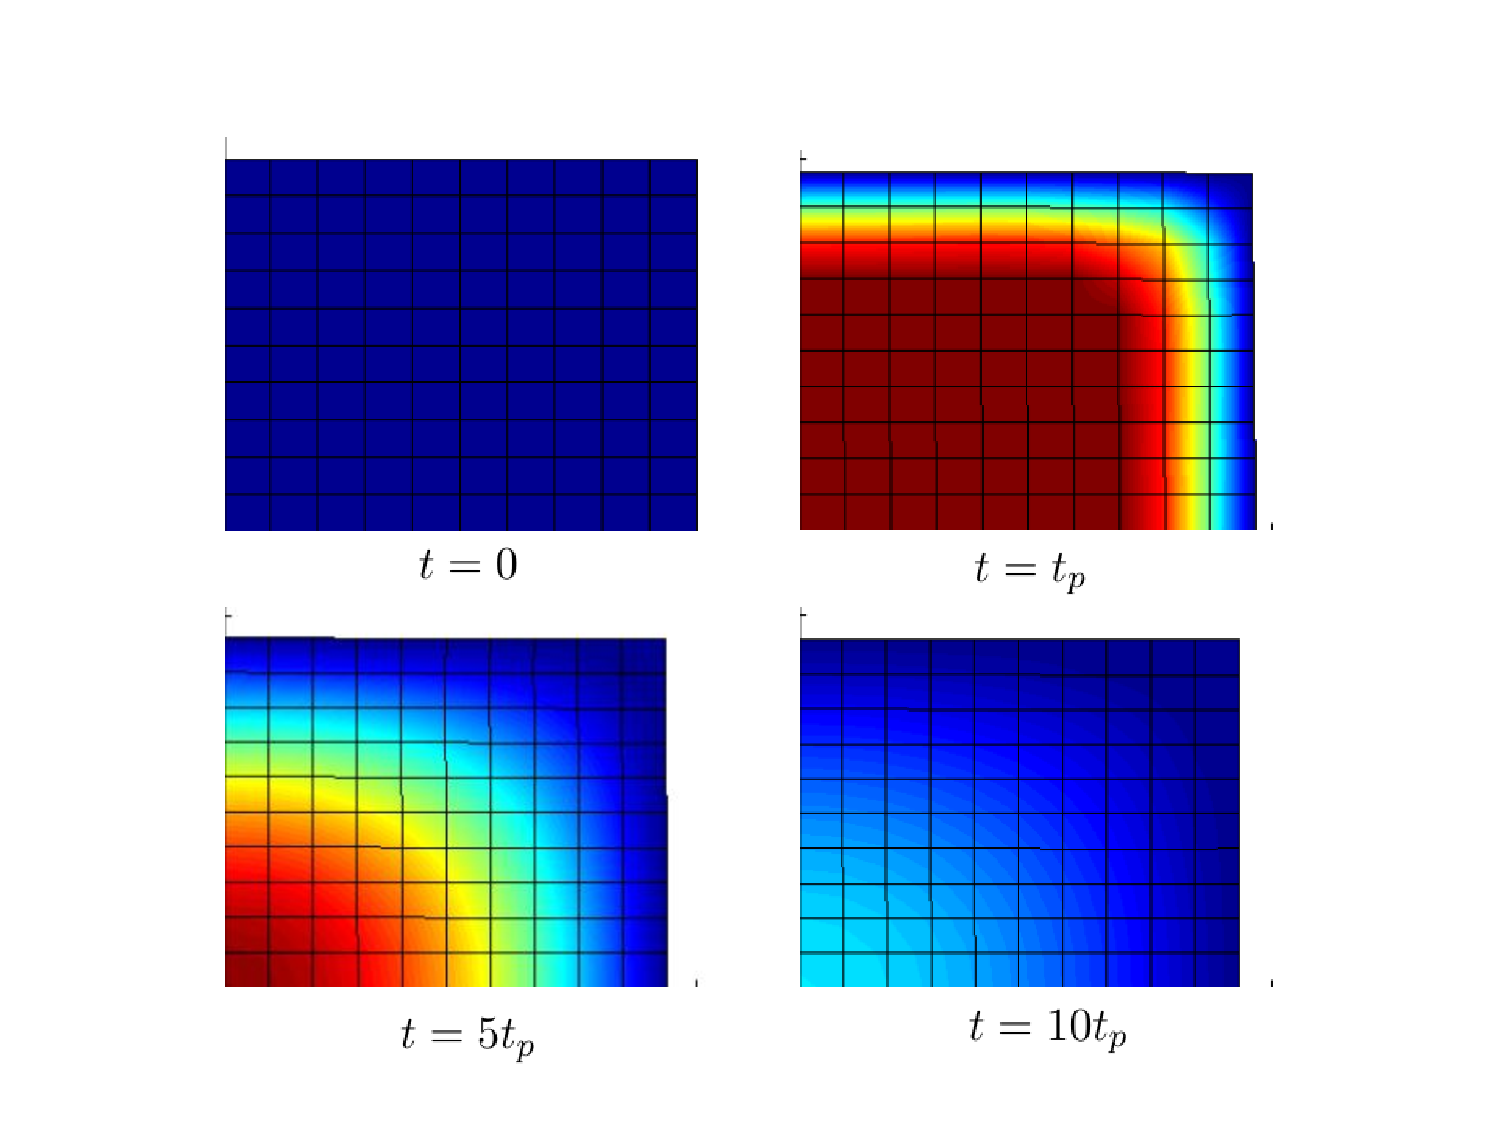
\includegraphics[width = 4.0in,trim=100 30 100 70,clip=true]{ramptest.pdf}
	\caption{MATLAB test problem for $P(t)$ defined in equation \ref{eq:rampload}}
	\label{fig:ramptest}
\end{figure}

As seen in figure \ref{fig:ramptest}, the domain has been discretized into a $10 \times 10$ Cartesian mesh. While we do not provide a color scale for the pressure values, blue may be thought of as $p = 0$, while red corresponds to the maximal value of $p$ attained for all time. Reviewing the results, we observe the effect of the increase in confining pressure between $t = 0$ and $t = t_p$ on the fluid pressure within the medium. Fluid pressures on $\partial_u B$ (the draining boundary) are of course seen to be equal to zero, but fluid pressures interior to the block of material reach a maximal plateau. The poroelastic skeleton is also observed to have compressed somewhat due to the external loading. For values of $t > t_p$, we see that the fluid pressure exhibits the diffusive behavior that we would expect, maintaining higher pressure at the center of the block of material (the lower-left portion of our quarter symmetry block) as the fluid slowly diffuses out along the draining boundary. Over time, the solution equilibrates back to a zero pressure state in the fluid, while the skeleton continues to compress as it begins to bear more of the total confining pressure. Qualitatively, this solution behavior agrees with our intuition, confirming that our development of the equations of poroelasticity produces a result that at least appears to be correct.

However, it is important that we consider the robustness of the method. In particular, we will examine a slightly different definition of $P(t)$ for our problem, such that
\begin{equation}
	P(t) = P \quad \forall t
	\label{eq:impulseload}
\end{equation}
This is equivalent to an impulsively applied external confining pressure at $t = 0$. The results are depicted in figure \ref{fig:impulsetest}.
\begin{figure} [!ht]
	\centering
	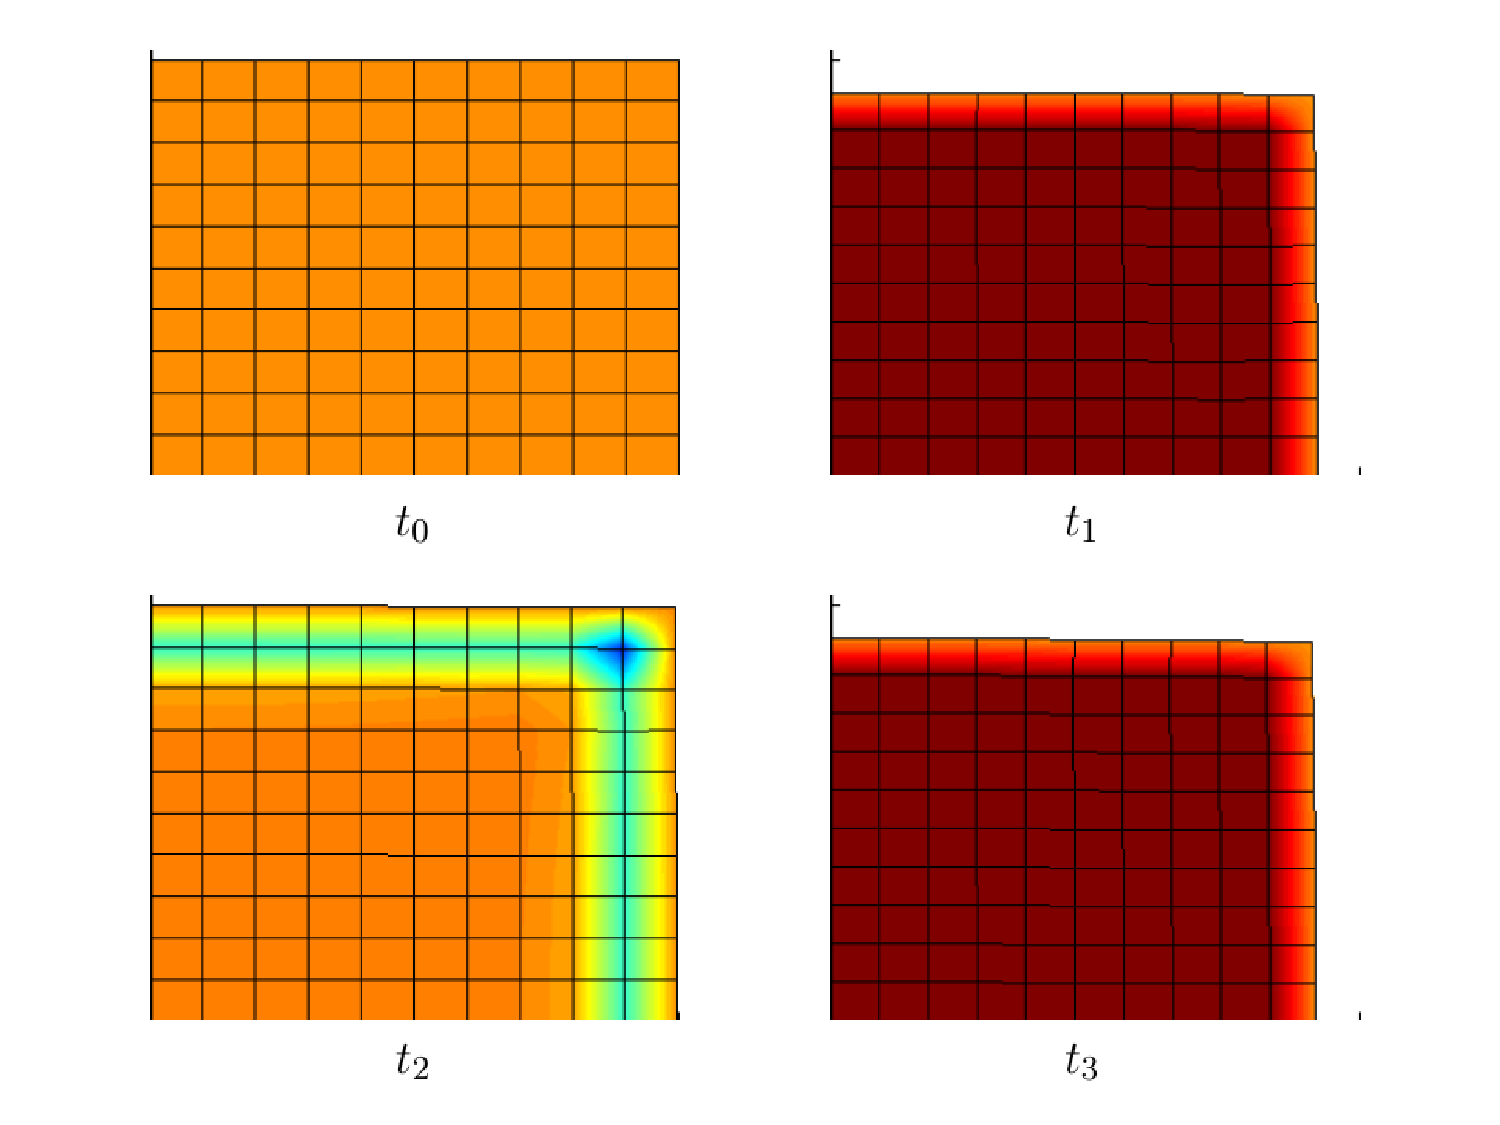
\includegraphics[width = 4.0in,trim=70 20 70 20,clip=true]{impulsetest.pdf}
	\caption{MATLAB test problem for $P(t)$ defined in equation \ref{eq:impulseload}}
	\label{fig:impulsetest}
\end{figure}

For the impulsive loading just described, we obtain spurious pressure oscillations in our solution, as seen from the first few times steps depicted in figure \ref{fig:impulsetest}. Clearly, our solution method is not entirely robust against certain choices of boundary and initial conditions. It should be stated that the oscillatory behavior of the pressure solution is a well-known issue with the coupled system of poroelastic equations (see references [9] and [10].) There exist a variety of techniques that have been successfully employed to mitigate this sort of behavior, among them the fluid pressure Laplacian stabilization (FPL) method described in reference [10]. FPL adds a stabilization term to the right-hand side of the weak form in equation \ref{eq:weakpressure}, namely
\begin{equation}
	B_{FPL} (q,p) = \int_B \tau q_{,i} k_{ij} \dot{p}_{,j} dv
\end{equation}
where $\tau$ is a selected stabilization parameter that involves the poroelastic constants, as well as a characteristic element length scale. For the time being, we will choose not to implement this stabilization technique, but we make note of the fact that our solutions may well encounter difficulties for certain choices of problem parameters. We leave the use of FPL stabilization as a topic for further research.

We will examine one last test problem for our MATLAB code before moving on to our implementation in GEOS. Specifically, we would like to see what would happen if we were to consider the same problem as shown in figure \ref{fig:ramptest}, but with the inclusion of a more permeable layer of material along the bottom edge of the quarter symmetry block. We define a spatially varying $\kappa(\mathbf{x})$ as
\begin{equation}
	\kappa(\mathbf{x}) =
	\left\{
	\begin{array}{ll}
		100\kappa & 0 \le x_2 \le h_e \\
		\kappa & h_e < x_2
	\end{array}
	\right.
	\label{eq:draink}
\end{equation}
where $h_e$ is the height of a single element in the mesh. This implies that the bottom layer of elements will have a permeability $100$ times greater than for the rest of the block of material. The results of this test are depicted in figure \ref{fig:draintest}.
\begin{figure} [!ht]
	\centering
	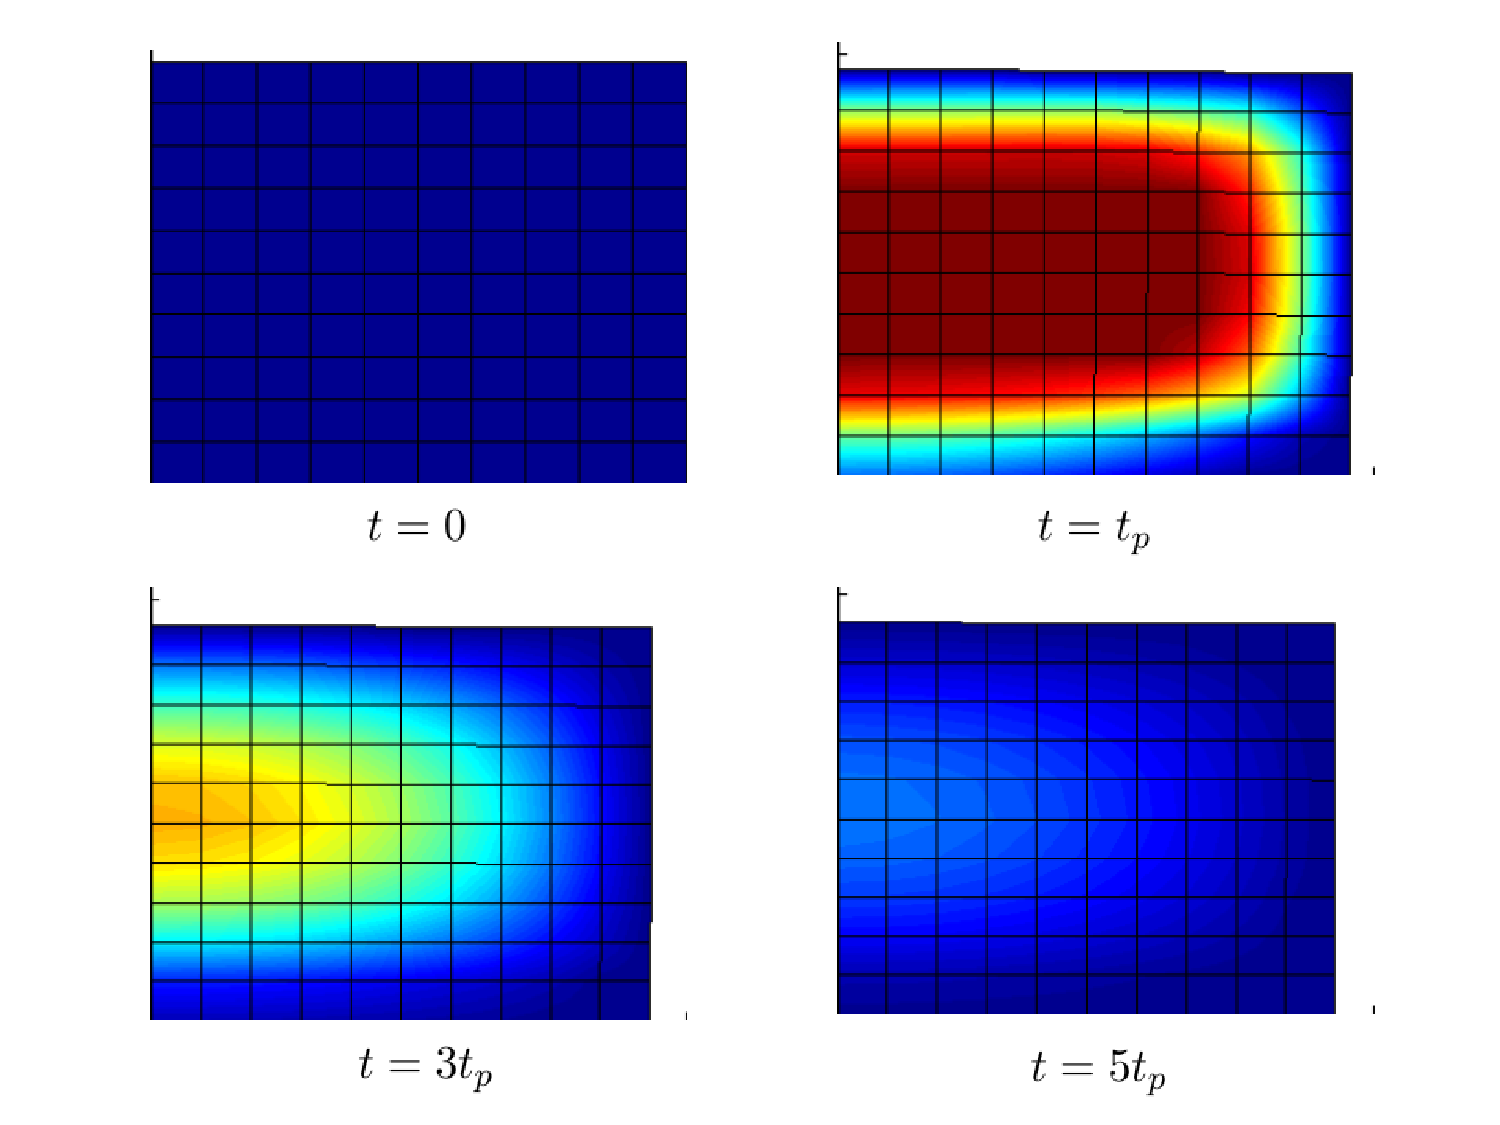
\includegraphics[width = 4.0in,trim=70 20 70 20,clip=true]{draintest.pdf}
	\caption{MATLAB test problem for $P(t)$ defined in equation \ref{eq:rampload}, and $k(\mathbf{x})$ defined in equation \ref{eq:draink}}
	\label{fig:draintest}
\end{figure}

The observed results in figure \ref{fig:draintest} appear to make intuitive sense. Because the saturating fluid is allowed to drain out of the material more easily in the permeable layer, it does not sustain as high of fluid pressures. As a result, the fluid within the rest of the block of material may either flow out of the exterior boundary, or through the draining layer. This result is significant, in that the behavior of the permeable layer emulates the behavior of a crack, which we would anticipate to more easily convey fluid. This suggests that perhaps a homogenized approach for modeling crack behavior may yet produce the results that we seek.

\newpage
\section{GEOS Implementation}

In what proceeds, we will elucidate the details of our poromechanics implementation within the GEOS code framework. We begin by briefly summarizing the existing accommodations for code development within GEOS, and our approach to the implementation.

GEOS is a C++ based code, developed for parallel computation of hydro-fracture problems. The existing framework of the code is designed to accommodate the addition of a variety of physics ``solvers'' (computation modules that are focused around the modeling of a specific type of physics.) A solver `object' is typically implemented as a C++ class. Different solvers may act as `base' classes, from which are derived more specific applications of a particular physics. For example, the `Lagrange' family of solvers all derive from a `LagrangeSolverBase' class, which by itself cannot be instantiated, as it contains a number of pure virtual functions. It is up to the derived classes (such as `LagrangeSmallStrainLinearElastic') to provide the implementation of these virtual methods contained in the base class. Apart from deriving from other classes, solvers may also be constructed as a `composition' of various sub-solvers. This is the case for many of the coupled solvers, which link the physics for the flow simulation to the physics of the solid deformation. For a particular problem, any number of physics solvers may be instantiated and used for the simulation, all of which are owned hierarchically by a ``problem manager'' object. It is the problem manager which organizes the overall finite element simulation for a particular problem, but it is the solvers which carry out the actual computations. This being the case, the creation of a poromechanics based physics solver is a likely place for us to begin our implementation.

Many of the high-level actions common to all physics solvers (such as determining the solution to a linear system of equations) are already implemented within the `SolverBase' class. This reduces some of the burden of creating a new solver from scratch, as we may inherit much of the basic functionality. As a first measure, we will need to specify certain quantities of interest for the poroelasticity problem. In particular, we may assign data to the nodes of a mesh, corresponding to the displacement and pressure degrees of freedom. We will also carry data for the incremental displacements and pressures at the nodes, as well. Global degree of freedom indicies are also associated with the nodes, which find their use in the assembly and solution of the full system of linear equations. We may also associate data with the elements of the mesh. Namely, we would like to assign certain fundamental poroelastic properties to individual elements, such as the skeleton stiffness parameters, porosity, and intrinsic permeability. From these (for the case of an isotropic poroelastic material,) we may determine the other properties, such as Biot's modulus and the fluid capacity. It would be preferable to associate these material properties with the integration points of the elements, but for the sake of keeping the formulation general and able to accommodate any number of different element types, we will forgo this approach. Parameters associated with the problem as a whole may be stored as data members of the solver object. These include values for $K_s$, $K_f$, $\rho_s^0$, $\rho_f^0$, $\sigma_t$, $\sigma_c$, and $g_i$, among others. A number of other solver-specific parameters (such as convergence tolerance and a maximum iteration number) can likewise be stored by the solver object.

At the level of the user interface, the solver needs to be capable of supporting appropriate specification of these aforementioned parameters and data fields for a given problem. GEOS parses problem input data through an user created XML file, which contains directives for the types of solvers to use, mesh data, node sets, boundary conditions, initial conditions, time variability, and output. Callable functions within the GEOS framework exist whose purpose is to facilitate reading this input data. These function calls can be made of use within our solver to incorporate the relevant problem parameters we need from user specified inputs.

The main body of computations performed by the solver involves the solution of a finite element system of equations for a given increment of time. Within a single time step, we will need to assemble a global residual vector, in addition to a global tangent `stiffness' matrix. We use the term `stiffness' in a loose way to refer generally to the derivative of the nodal residual, though the $\textbf{K}_{uu}$ portion of this total matrix is the only quantity truly deserving of being called a stiffness matrix. To this end, we may perform a loop over the total number of elements in the mesh, collecting the necessary parameters and field data to be able to compute the local element residual and derivative using the incremental pressure and displacement form of equation \ref{eq:matrixequations}. At the element level, the equation assembly takes place by first looping over the number of quadrature points $q$, looping over the nodes of the current element for index $a$, and once again over the nodes for index $b$. GEOS already has in place a library of element classes that will provide us with precomputed shape function values, their gradients, and values of the Jacobian determinant at the quadrature points. With these in hand, we can carry out the integrals described in equations \ref{eq:Kuu} through \ref{eq:Mpp} and equations \ref{eq:Fu} through \ref{eq:Fp2}. These element contributions can then be summed into the global system of equations. It may be of interest to note that in our global system of equations (for $\mathbf{u} \in \rm I\!R^3$,) the $u_1$, $u_2$, and $u_3$ displacement degrees of freedom for node $a$ will be stored in the global degree of freedom array with indicies $3a$, $3a + 1$, and $3a + 2$, respectively, with the pressure degree of freedom $p$ being stored in the $3a + 3$ global index (for C++ indexing from $0$.)

The assignment of appropriate essential and natural boundary conditions may be handled using some of the existing implementation used in other, similar solvers. For the essential boundary conditions (fluid pressures and skeleton displacements) we may borrow much of the same techniques used for specification of solid displacements used in the Lagrange family of solvers. This effectively involves zeroing out the equation rows corresponding to the constrained degrees of freedom for the problem within our global system of equations. The corresponding `dof' values in the global residual vector can then be replaced by the prescribed displacement or pressure values, with the diagonal entires in the global `stiffness' matrix for these entires set equal to $1$. An appropriate scaling of these equation rows would need to be performed. For the natural boundary conditions, we would need to perform surface integrals over element facets on the boundary of the body. An existing scheme for computing traction boundary condition contributions to the nodal residual may be utilized, and further adapted for the case of a prescribed flux boundary condition.

As alluded to previously, the solution of the resulting system of poroelasticity equations (for the incremental pressures and displacements) can be solved using the existing linear solver packages. Though we may extensibly make use of the Trilinos iterative solvers available for use, for debugging purposes we will choose only to use a direct linear solver. Ideally, we would pursue a time stepping scheme in which we select an appropriate stable time step size in an effort to avoid the spurious pressure oscillations seen in our MATLAB implementation. However, for the sake of simplicity, we will only allow for a constant user-specified time step value to be used.

For the incorporation of our local damage mechanics model, we will need to introduce an outer Newton-Raphson iteration loop within a given time step that will progressively evolve the damage variables within each element according to the algorithm described in section 4. From the norm of equation \ref{eq:oldnorm}, we more explicitly select a max norm over the elements $e$, such that
\begin{equation}
	\max_e \frac{| D^e_{i+1} - D^e_{i} |}{D^e_{i}} < tol
\end{equation}
which should mitigate the worst-case relative error in the damage variable for a given Newton-Raphson iteration.

With our poromechanics solver in place, we now examine a few test problems to verify the correctness of our implementation, as well as demonstrate the capabilities and limitations of our approach for modeling hydro-fracture problems.

We begin by exploring an identical problem to the one described for our MATLAB implementation, now in the case of three dimensions. Instead of modeling a single quadrant of a two-dimensional block of poroelastic material suspended in a zero-pressure fluid, we model a single octant of a three-dimensional cube placed under similar conditions. As was the case for our MATLAB test problem, we will apply an external confining pressure to the poroelastic cube (the positive $x$, $y$, and $z$ faces,) using a definition for $P(t)$ as in equation \ref{eq:rampload}. The results (generated with the VisIt visualization tool) are depicted in figure \ref{fig:cubetest}.

\begin{figure} [!ht]
	\centering
	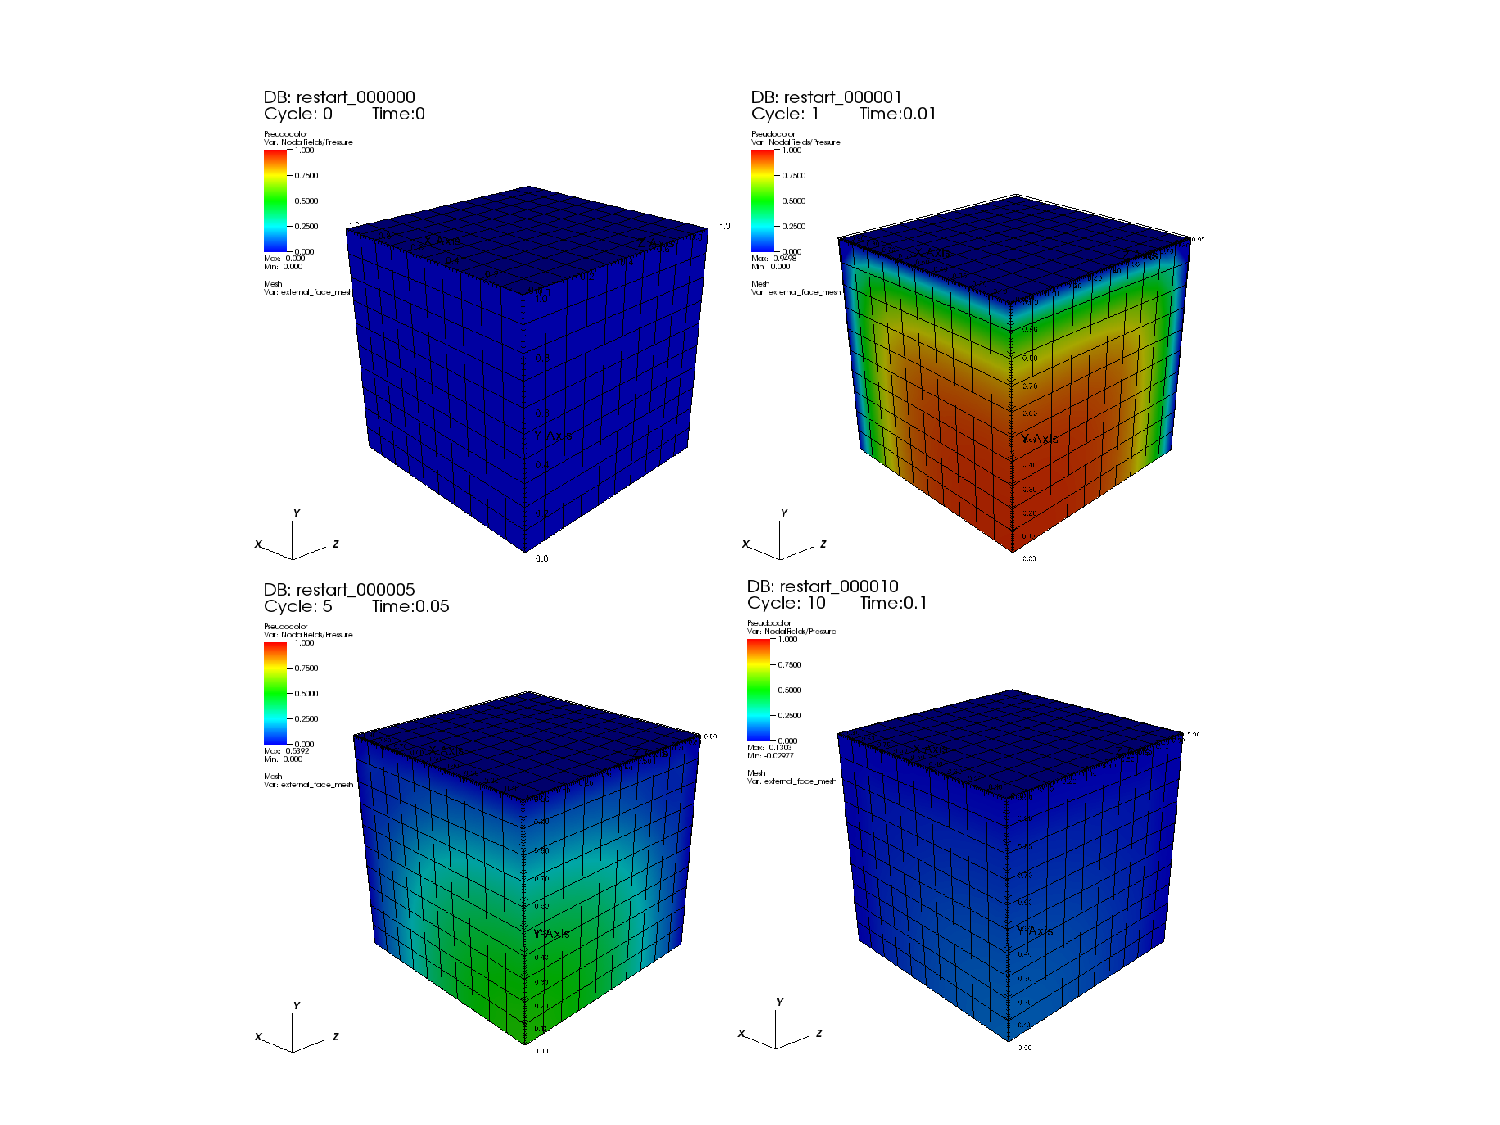
\includegraphics[width = 5.0in,trim=120 30 140 40,clip=true]{cubetest.pdf}
	\caption{Poroelastic cube subjected to a confining pressure. Plotted results for the fluid pressure on the deformed mesh at selected times.}
	\label{fig:cubetest}
\end{figure}

As we would hope, the qualitative results are very much the same as what we obtained for the two-dimensional MATLAB test problem. Though we will not show the plotted results for the case when $P(t)$ is specified to be an impulsively applied confining pressure, we note that the same pressure oscillations in the solution are present as for the MATLAB test problem. The implementation of a fluid pressure stabilization term is left as a subject for further development, but will not be pursued at this time. It is sufficient for our purposes at the moment to only explore problems in which the problem parameters produce stable results. Though it is difficult to say with absolute certainty that the implementation correctly models the true physical process, we take these results as sufficient evidence that the poromechanics component of our solver is working properly, or at least as expected. However, the efficacy of the damage mechanics portion is yet to be determined.

Therefore, we endeavor to devise an appropriate test problem that will help to give us an idea of whether our material damage model produces desirable results. In the interest of being able to visualize the result more easily, we will explore a simple two-dimensional problem. Again, we will define a square block of homogeneous and isotropic poroelastic material. The skeleton displacements normal to the entire boundary of the problem will be assigned zero value, effectively constraining the block of material from expanding. Zero flux will be prescribed on all external facets, with the exception of the right-hand edge of the block. To this face, we will assign all zero fluid pressure boundary conditions, with the exception of a small collection of facets near the bottom edge which will have a non-zero, inward directed fluid flux. These boundary conditions are represented pictorially in figure \ref{fig:cracktestbcs}.

\begin{figure} [!ht]
	\centering
	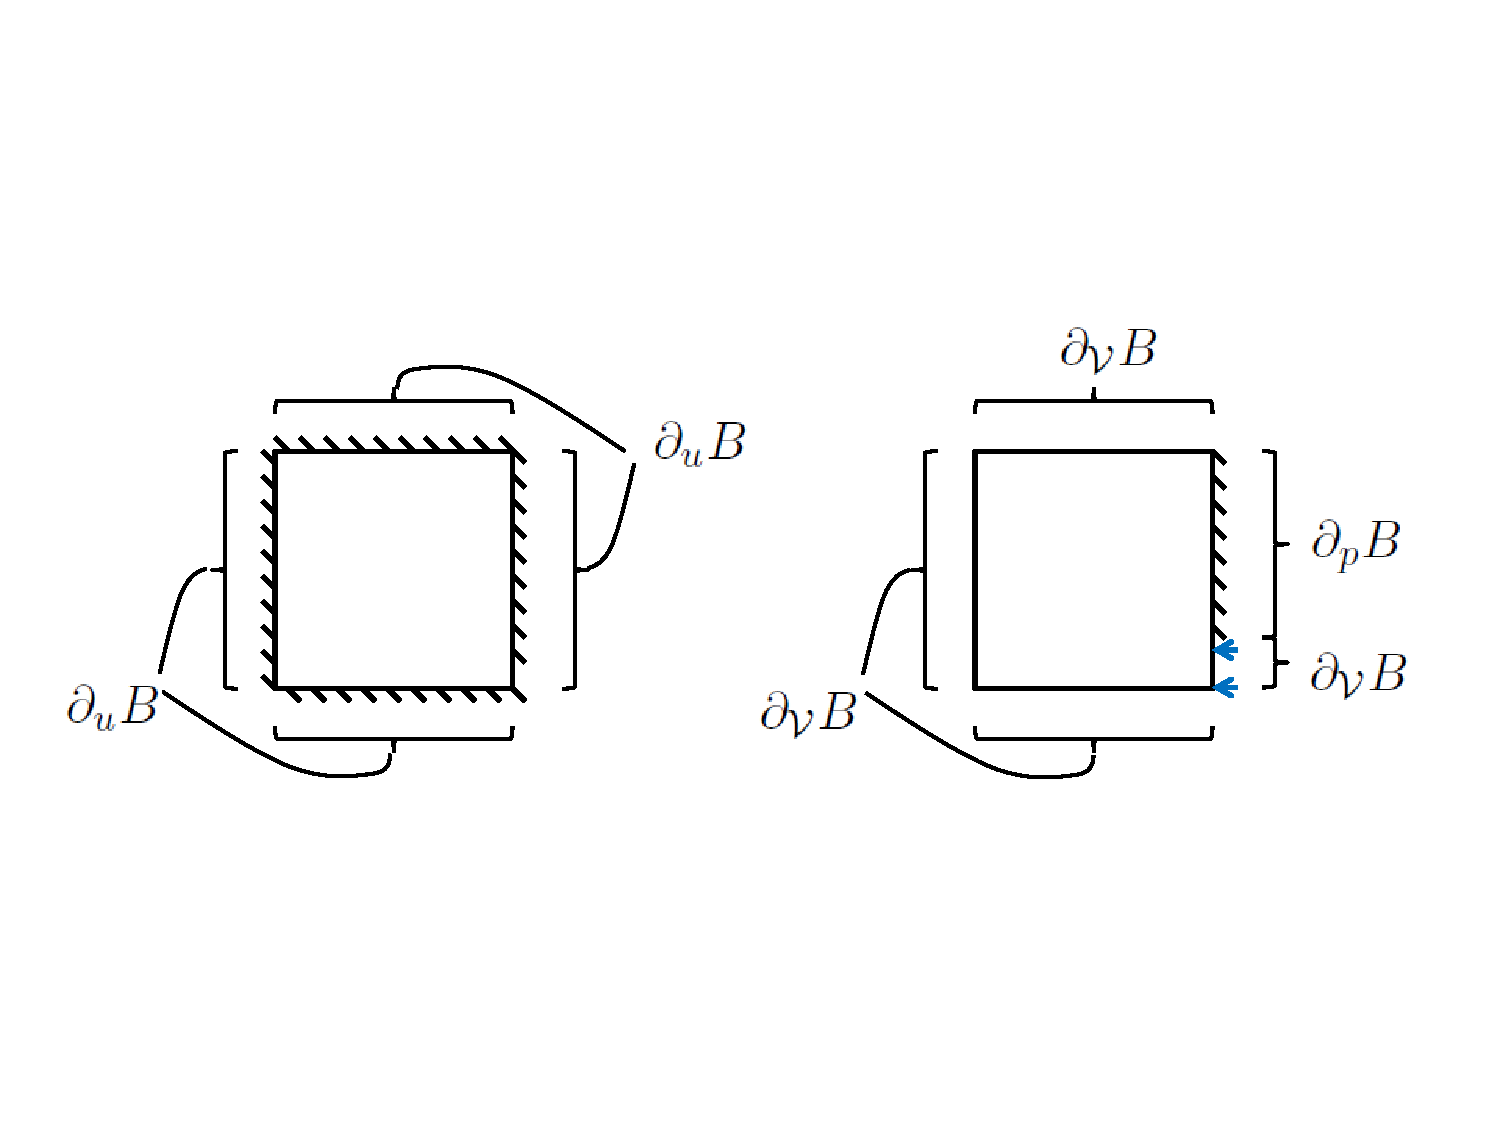
\includegraphics[width = 4.0in,trim=30 160 40 150,clip=true]{cracktest.pdf}
	\caption{Boundary conditions for damage mechanics test problem}
	\label{fig:cracktestbcs}
\end{figure}

Physically, we may conceive of the problem as being one where we are injecting fluid over a small region into a confined block of material. If the fluid injection rate is high enough, then it should be possible for us to induce material failure. To more accurately emulate the fracture behavior of rock, we will set the tensile failure stress to be much less than the compressive failure stress ($\sigma_t << \sigma_c$.) Running this problem at a fairly coarse refinement level, we obtain the results depicted in figures \ref{fig:lowdamage} and \ref{fig:lowpressure}.

\begin{figure} [!ht]
	\centering
	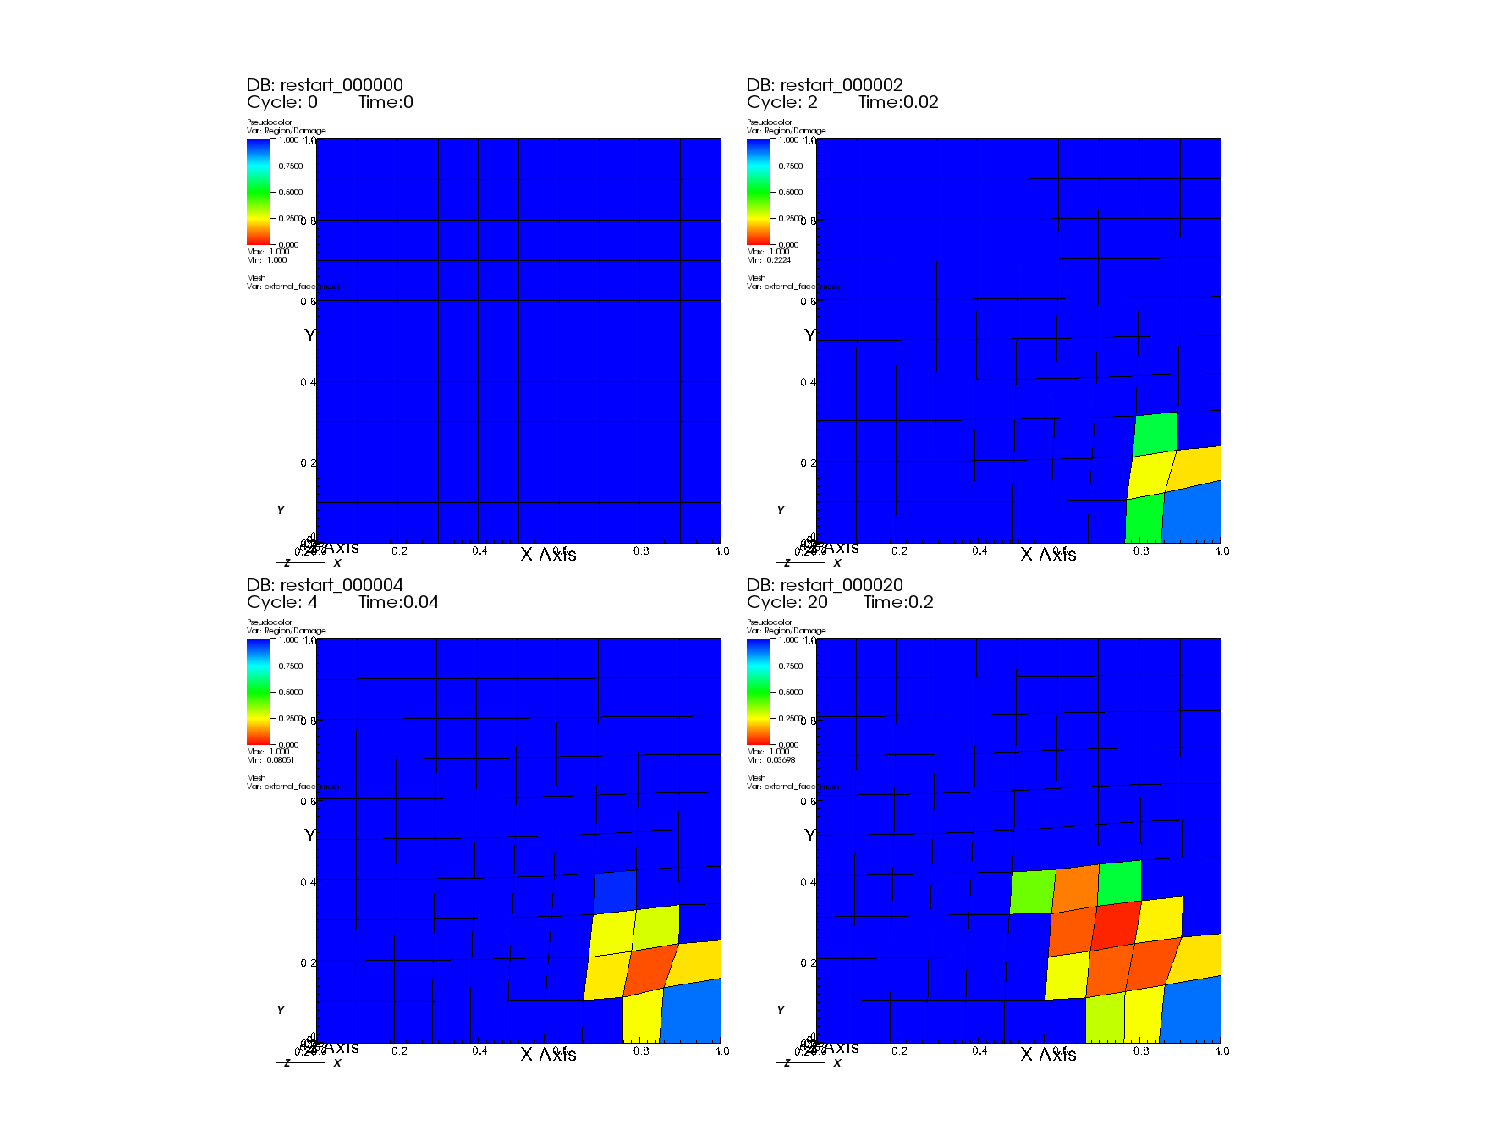
\includegraphics[width = 5.0in,trim=110 20 130 30,clip=true]{lowdamage.pdf}
	\caption{Damage mechanics test problem for a $10 \times 10$ mesh. Plotted results for the damage variable $D$ on the deformed mesh at selected times.}
	\label{fig:lowdamage}
\end{figure}

\begin{figure} [!ht]
	\centering
	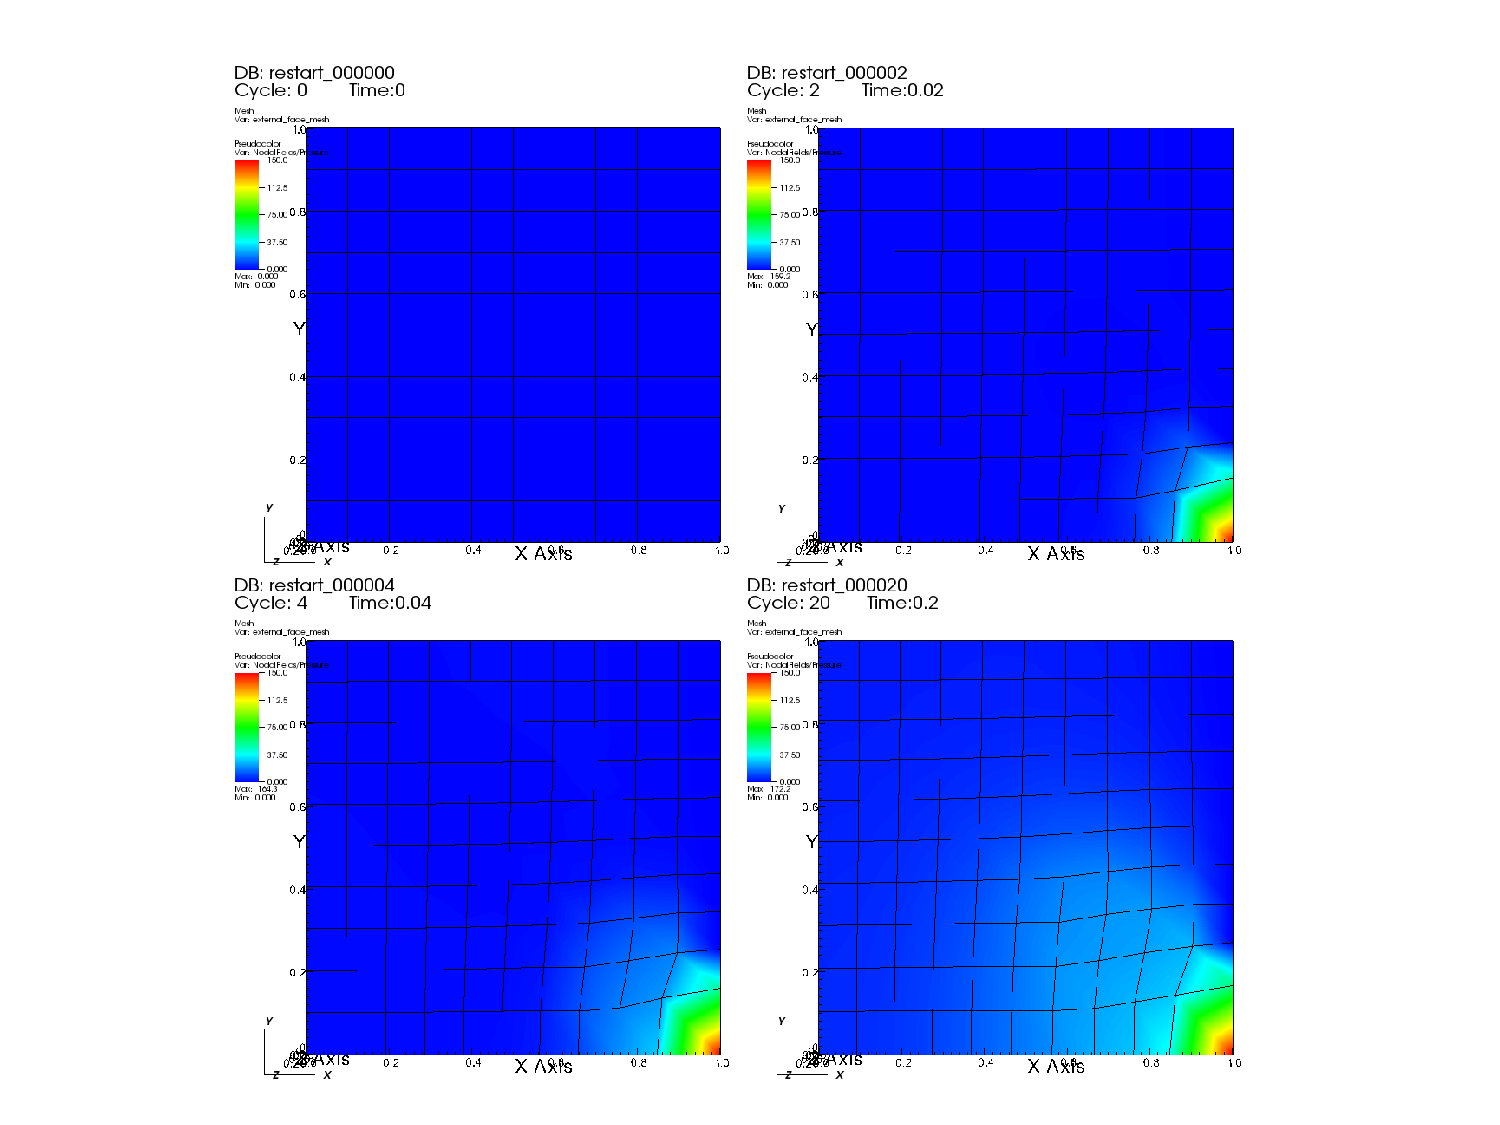
\includegraphics[width = 5.0in,trim=110 20 130 30,clip=true]{lowpressure.pdf}
	\caption{Damage mechanics test problem for a $10 \times 10$ mesh. Plotted results for the fluid pressure $p$ on the deformed mesh at selected times.}
	\label{fig:lowpressure}
\end{figure}

In figure \ref{fig:lowdamage}, we observe that the extent of damage in the material does appear to propagate in a crack-like fashion, initiating at the bottom-right hand corner, and progressing inward toward the center of the block. However, there does appear to be some strange behavior in the bottom-rightmost element of the mesh, which despite being the most dilated element, it does not appear to have received as much damage as one might expect. It is important to remark that our failure criterion was developed to produce fracture within elements experiencing high deviatoric stresses. However, given that the bottom-rightmost element has many of its displacement degrees of freedom constrained, it is not allowed to deform in a manner that would produce shear strains within the element. This may explain why this element in particular has received less damage than the elements interior to the body, which are seen to deform primarily in shear, as we would anticipate. A similar phenomenon may explain why the elements with constraints on the bottom and right edges of the body are also less damaged, despite their proximity to the fluid injection site. It is also important to note that our implementation of the damage algorithm only considered the \textit{averaged} strain within the element, since we chose to associate only a single damage variable with a given element. We may well be able to improve our results if we instead consider the evolution of damage at individual integration points. This perhaps indicates some issues with our damage model as it is currently implemented, which may provide opportunities to make future improvements, though we choose not to pursue them at present.

We confirm that the crack is fluid pressure-driven by observing the results in figure \ref{fig:lowpressure}, which shows zones of increased fluid pressures in the same locations as the damaged zones. We may conceive of the crack `front' as being located where there is a sufficient fluid pressure gradient. Elements at the crack front receive a high influx of fluid, which results in a fluid pressure increase. This results in a corresponding decrease in the skeleton effective pressure, inducing material failure. As the element becomes more damaged, its hydraulic conductivity increases, allowing for fluid to pass more easily through it, relieving the high pressure gradient. This results in the crack front being extended to the adjacent elements, who in turn become damaged, thus resulting in a behavior that emulates crack propagation. However, it is difficult to distinguish a crack tip from a fractured face within the material, particularly for the isotropic material degradation scheme which we have chosen to pursue. Since there will also be a high pressure gradient in directions normal to the crack plane, there is little that differentiates a true crack tip from the rest of the boundary of the entire damaged zone. This signals a need for further exploration of anisotropic material degradation schemes, in which we might consider (in addition to the damage parameter) a vector quantity indicating a crack normal direction. This can then be used to degrade the material properties orthotropically (in the plane of the presumed crack,) only allowing increased fluid flow to occur within this plane, and not in the crack normal direction. This might help aid in resolving a crack tip, but it presents difficulties if one were to desire the intersection of multiple cracks at differing angles. These are left as topics to be explored in future work.

To test whether our results are influenced by the mesh size, we will explore the same problem at a higher grid refinement level (now $20 \times 20$, rather than the original $10 \times 10$ mesh.) The corresponding plots of the damage and pressure variables are depicted in figures \ref{fig:highdamage} and \ref{fig:highpressure}, respectively.

\begin{figure} [!ht]
	\centering
	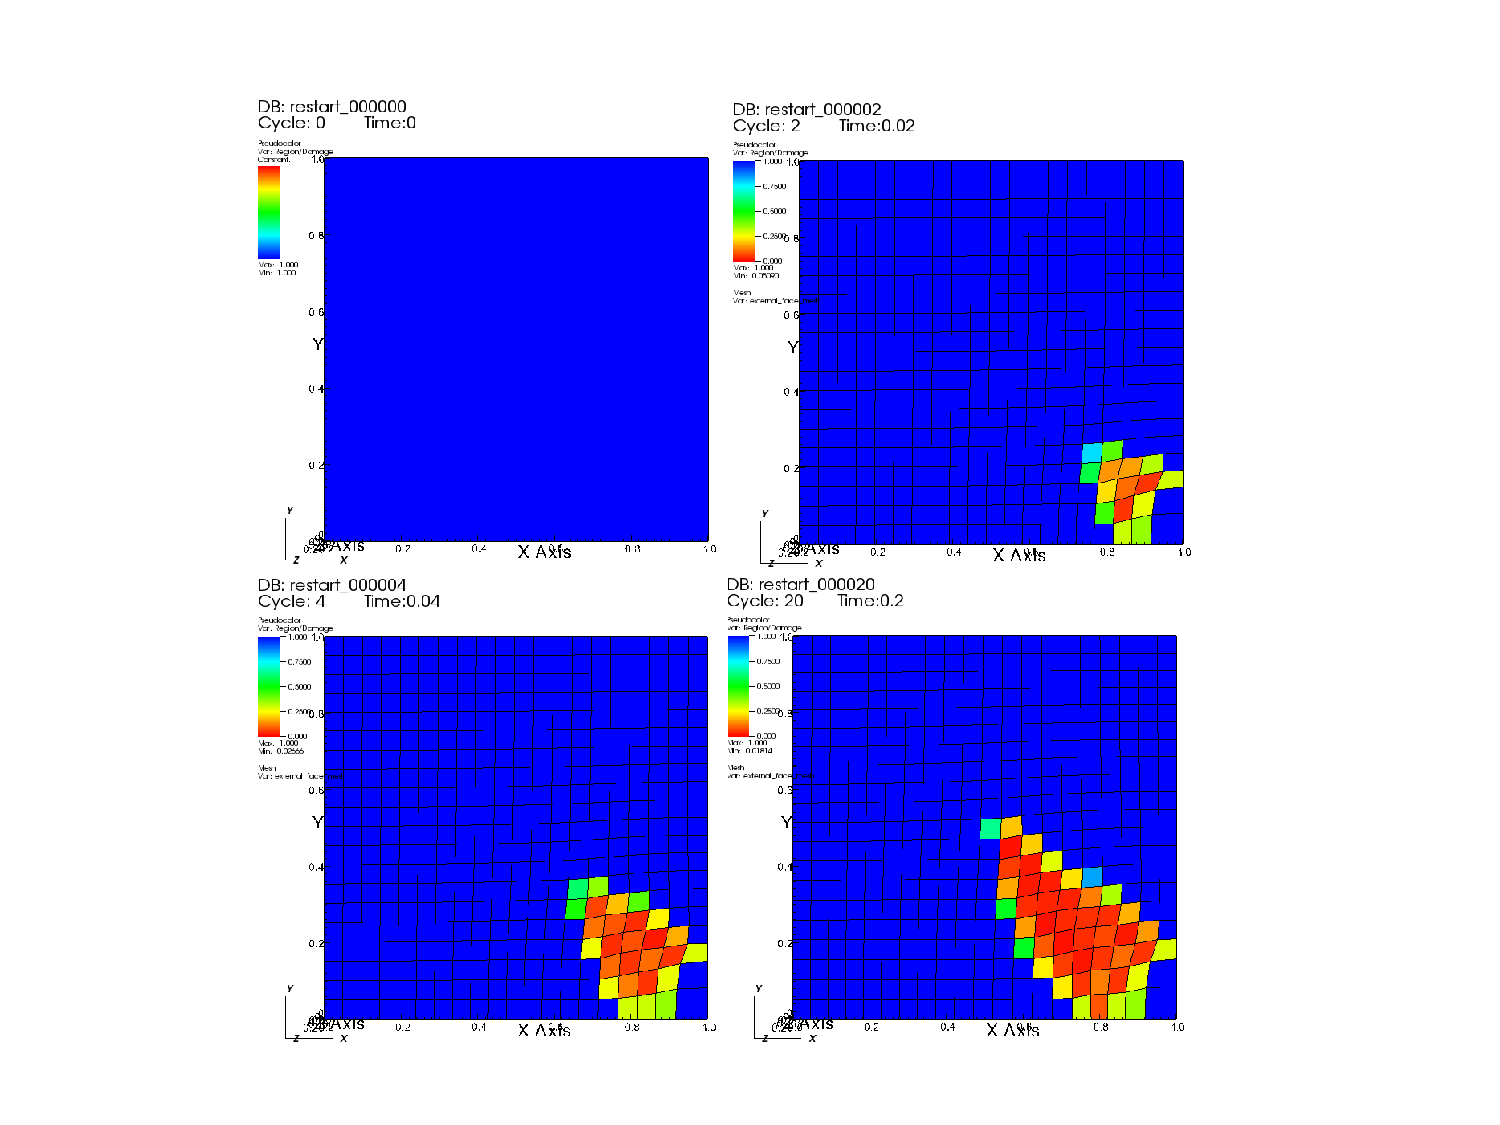
\includegraphics[width = 5.0in,trim=110 20 130 30,clip=true]{highdamage.pdf}
	\caption{Damage mechanics test problem for a $20 \times 20$ mesh. Plotted results for the damage variable $D$ on the deformed mesh at selected times.}
	\label{fig:highdamage}
\end{figure}

\begin{figure} [!ht]
	\centering
	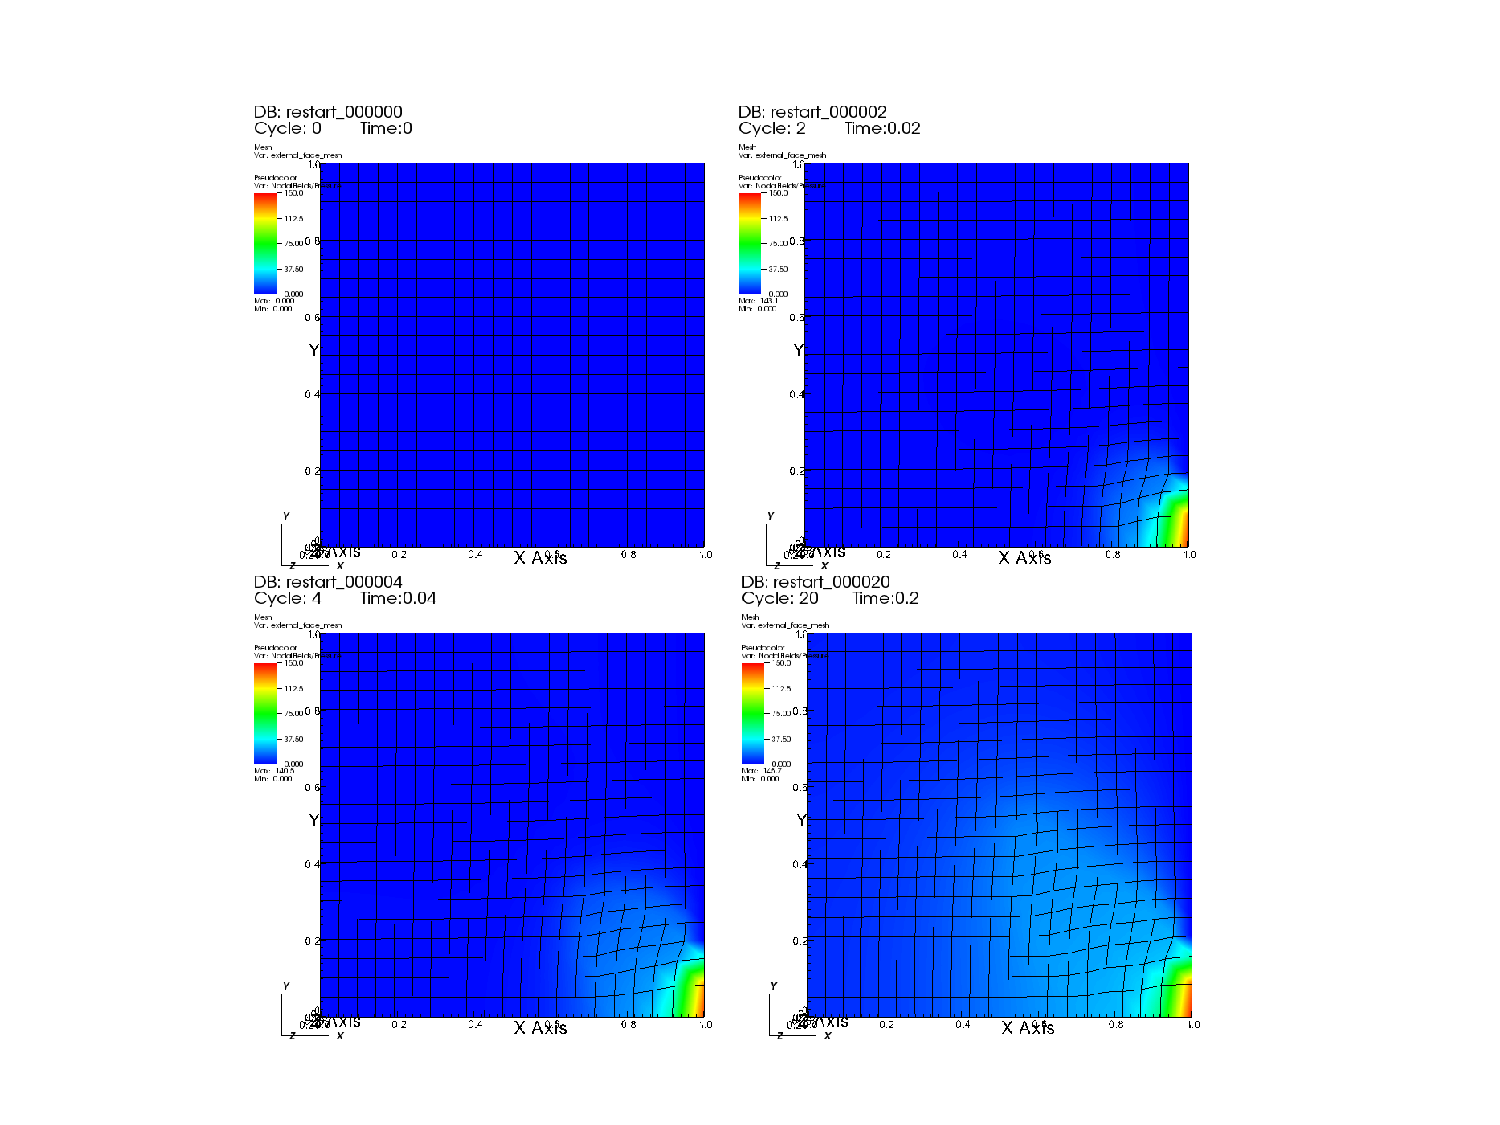
\includegraphics[width = 5.0in,trim=110 20 130 30,clip=true]{highpressure.pdf}
	\caption{Damage mechanics test problem for a $20 \times 20$ mesh. Plotted results for the fluid pressure $p$ on the deformed mesh at selected times.}
	\label{fig:highpressure}
\end{figure}

Despite some minor discrepancies (particularly near the fluid injection site,) the results appear to scale reasonably well at a higher resolution, maintaining much of the same macroscopic characteristics observed for the $10 \times 10$ refinement level. The extent of damage is observed to be much more localized and severe for individual elements, but this would seem to agree with our conception of a homogenized crack becoming `smeared' out in a coarser mesh. The behavior of the fluid pressure similarly conforms to our previously stated expectations. Now, however, we can see a more sharply defined crack boundary, corresponding to a much sharper pressure gradient within individual elements. It may be speculated that further resolution of the crack boundary may be had if we further refine the mesh.

Though these results are encouraging, they do raise some concerns surrounding adequate representation of the crack. Ideally, we would prefer crack `width' to become smaller as we refine the mesh, localizing to only a small band of elements. However, this does not appear to be the case for our damage model. This may be attributed to the isotropic degradation. Since damage does not occur in any preferential direction, the `width' of cracks may become arbitrarily large. It may be postulated that for an anisotropic damage scheme, we may be able to alleviate this problem. But once again, this will be a topic left open for further development.

\section{Conclusions and Future Work}

Based on the results obtained through the limited number of test problems we observed, it is clear that significant work still would need to be done before such an approach would be reasonable for modeling large-scale hydro-fracture problems.

In particular, our damage model would likely be the component in most need of improvement. As suggested in the previous section, the development of an anisotropic damage scheme would be an appropriate first step to this end. This would hopefully resolve some of the issues surrounding the proper identification of crack tips, and the limiting of crack widths under mesh refinement. Another issue to consider would be the differentiation between crack initiation versus crack propagation. Ideally, crack initiation should occur at a much higher stress level than crack propagation, but our present model makes no distinction between the two. This might be cause for the development of an appropriate fracture initiation criteria, that may well necessitate a non-local approach in which we would check for the locality of a crack tip in adjacent elements. Cohesive zone elements may also be topic to consider, but this assumes that we would be able to properly identity crack tips.

We might also consider revising the nature of the material degradation. We note that in keeping the bulk modulus of the skeleton constant while degrading the shear modulus, this would result in the ratio of $K/G$ approaching infinity as the damage variable $D$ goes to $0$. In other words, this would be equivalent to the poroelastic material approaching the incompressible limit, which would lead to the notorious issue of volumetric locking. For this reason, it would be of necessity for us to find a way to alleviate this problem, possibly through a mixed/penalty approach in the element formulation. Otherwise, we might consider placing a lower limit on the damage variable to prevent this from becoming an issue.

Given the true physical behavior of the cracks, we might also desire the material deformation to behave in a manner more akin to a typical plasticity model, which may have pressure-dependent stiffness properties. Since we may think of the cracks as likely being jagged surfaces, a compressed region of cracked rock should therefore still maintain the majority of its shear stiffness. A slipping of two surfaces along a given crack plane could be conceived of as a kind of `crack strain,' much akin to a plastic strain, which would be altogether separate from the elastic strain. In this way, slippage along cracks could occur only so long as there is sufficient fluid pressure to force the crack opening. However, if the fluid pressure were to decrease, we would expect the crack to close, and for the material to enter back into an elastic region (albeit now shifted by the total cracked strain.) To overcome the jagged surfaces of the cracked faces, we might also anticipate some dilational behavior of the rock during slippage, in the same way that a compacted sand would dilate during shear deformation. It may then be of interest to perhaps adapt plasticity models typically associated with sands for application within our own damage model.

Though the basic physics behavior of the poromechanics component of our solver appears to work reasonably well for certain choices of problem parameters, we still would likely need to implement some form of fluid pressure stabilization. High pressure oscillations in the solution could lead to the initiation or propagation of cracks that might not otherwise occur. For this reason, a lack of pressure stabilization may prove to be a significant issue for certain problems. A fully dynamic, finite deformation formulation of poromechanics may also yield more robust results, in that the dynamics of the poroelastic skeleton may be of assistance in stabilizing the fluid pressures.

Following some of the aforementioned improvements, we might find ourselves in an appropriate position to deem whether a homogenized approach is adequate for modeling hydraulic fracture problems. Such claims may hopefully be established in future work.

\newpage

\section{References}
\begin{itemize}
	\item[{[1]}] Anandarajah, A. \textit{Computational Methods in Elasticity and Plasticity Solids and Porous Media.} New York: Springer, 2010. Print.
	\item[{[2]}] Boone, Thomas J., and Anthony R. Ingraffea. ``A Numerical Procedure for Simulation of Hydraulically-driven Fracture Propagation in Poroelastic Media.'' \textit{International Journal for Numerical and Analytical Methods in Geomechanics} 14.1 (1990): 27-47. Web.
	\item[{[3]}] Chow, C.l., and F. Yang. ``On One-parameter Description of Damage State for Brittle Material.'' \textit{Engineering Fracture Mechanics} 40.2 (1991): 335-43. Web.
	\item[{[4]}] Coussy, Olivier. \textit{Poromechanics.} Chichester, England: Wiley, 2004. Print.
	\item[{[5]}] Hughes, Thomas J. R. \textit{The Finite Element Method: Linear Static and Dynamic Finite Element Analysis.} Englewood Cliffs, NJ: Prentice-Hall, 1987. Print.
	\item[{[6]}] Gajo, A., and R. Denzer. ``Finite Element Modelling of Saturated Porous Media at Finite Strains under Dynamic Conditions with Compressible Constituents.'' \textit{International Journal for Numerical Methods in Engineering} 85.13 (2011): 1705-736. Web.
	\item[{[7]}] Hamiel, Y., V. Lyakhovsky, and A. Agnon. ``Coupled Evolution of Damage and Porosity in Poroelastic Media: Theory and Applications to Deformation of Porous Rocks.'' \textit{Geophysical Journal International} 156.3 (2004): 701-13. Web.
	\item[{[8]}] Pasquale, Giovine. ``A Mixture Theory for Microstructured Porous Media.'' \textit{ZAMM - Journal of Applied Mathematics and Mechanics / Zeitschrift Für Angewandte Mathematik Und Mechanik} 80.S1 (2000): 153-56. Web.
	\item[{[9]}] Phillips, Phillip Joseph. \textit{Finite Element Methods in Linear Poroelasticity Theoretical and Computational Results.} Thesis. University of Texas at Austin, 2005. N.p.: n.p., n.d. Print.
	\item[{[10]}] Preisig, Matthias, and Jean H. Prévost. ``Stabilization Procedures in Coupled Poromechanics Problems: A Critical Assessment.'' \textit{International Journal for Numerical and Analytical Methods in Geomechanics} 35.11 (2011): 1207-225. Web.
	\item[{[11]}] Settgast, Randolph, Scott Johnson, Pengcheng Fu, Stuart D.C. Walsh, and Frederick Ryerson. ``Simulation of Hydraulic Fracture Networks in Three Dimensions.'' \textit{Proceedings of the Thirty-Sevenths Workshop on Geothermal Reservoir Engineering} (n.d.): n. pag. Web.
	\item[{[12]}] Showalter, R. E., and Bahareh Momken. ``Single-phase Flow in Composite Poroelastic Media.'' \textit{Mathematical Methods in the Applied Sciences} 25.2 (2002): 115-39. Web.
\end{itemize}

\end{document}
